\documentclass[xcolor={dvipsnames,table},aspectratio=169]{beamer}
\usepackage[utf8]{inputenc}
\usepackage[T1]{fontenc}

\usepackage[listings,minted,skins]{tcolorbox}
% \tcbuselibrary{skins}
\newtcblisting{myjava}{listing engine=minted,minted style=colorful,minted language=java,minted options={fontsize=\small,breaklines,autogobble,linenos,numbersep=3mm},
colback=blue!5!white,colframe=blue!75!black,listing only,
left=5mm,enhanced,
overlay={\begin{tcbclipinterior}\fill[red!20!blue!20!white] (frame.south west)
rectangle ([xshift=5mm]frame.north west);\end{tcbclipinterior}}}

\usepackage[brazil]{babel}
\usepackage{graphics,amssymb,amsfonts,amsmath}
\usepackage{tikz}
\usepackage{enumerate,hyperref}
\usepackage{palatino}
\usepackage{ragged2e}
\usepackage{minted}
\usepackage{booktabs}
\usepackage{verbatim}
\usepackage[export]{adjustbox}
\usepackage{tikz}                   
\usepackage{xcolor}
\usepackage{textcomp} % para usar \textdegree
\usetikzlibrary{shadows}
\usetheme{AnnArbor}
\usecolortheme{orchid}
\usefonttheme[onlymath]{serif}

\newcommand\setItemnumber[1]{\setcounter{enumi}{\numexpr#1-1\relax}}

\AtBeginSection[]{
  \begin{frame}
  \vfill
  \centering
  \begin{beamercolorbox}[sep=8pt,center,shadow=true,rounded=true]{title}
    \usebeamerfont{title}\insertsectionhead\par%
  \end{beamercolorbox}
  \vfill
  \end{frame}
}

\newminted{java}{bgcolor=cyan!10}

\newcolumntype{C}[1]{>{\centering\let\newline\\\arraybackslash\hspace{0pt}}m{#1}}

\title[\sc{Arrays}]{Arrays}
\begin{comment}
\title[\sc{Arrays e Array Lists}]{Arrays e Array Lists}
\end{comment}
\author[Roland Teodorowitsch]{Roland Teodorowitsch}
\institute[FPROG - EP - PUCRS]{Fundamentos de Programação - Escola Politécnica - PUCRS}
\date{22 de maio de 2023}

\begin{document}
\justifying

%-------------------------------------------------------
\begin{frame}
	\titlepage
\end{frame}

%=======================================================
\section{Introdução}

%-------------------------------------------------------
\begin{frame}\frametitle{Objetivos}
\begin{itemize}
%	\item Coletar elementos usando \emph{arrays} e \emph{array lists}
	\item Coletar elementos usando \emph{arrays}
%	\item Usar o laço \texttt{for} abreviado para percorrer \emph{arrays} e \emph{array lists}
%	\item Usar o laço \texttt{for} abreviado para percorrer \emph{arrays}
%	\item Aprender os algoritmos comuns para processamento de \emph{arrays} e \emph{array lists}
	\item Aprender os algoritmos comuns para processamento de \emph{arrays}
	\item Trabalhar com \emph{arrays} bidimensionais
	\item Receber e processar argumentos da linha de comandos
\end{itemize}
\end{frame}

%-------------------------------------------------------
\begin{frame}\frametitle{Conteúdos}
\begin{itemize}
	\item \emph{Arrays}
	\item Algoritmos Comuns para \emph{Arrays}
	\item Usando \emph{Arrays} com Métodos
	\item Tópicos Especiais
	\item Solução de Problemas
	\begin {itemize}
		\item Combinando Algoritmos
		\item Usando Objetos Reais
	\end{itemize}
	\item \emph{Arrays} Bidimensionais
%	\item \emph{Array Lists}
	\item Argumentos da Linha de Comando
	\item Sumário
	\item Humor
	\item Tópicos complementares
	\item Referências
\end{itemize}
\end{frame}

%=======================================================
\section{Arrays}

%-------------------------------------------------------
\begin{frame}\frametitle{\emph{Arrays}}
\begin{itemize}
	\item Um programa de computador frequentemente necessita armazenar uma lista de valores para então processá-los
	\item Por exemplo:
	\begin{itemize}
		\item Cálculo de variância ou desvio padrão
		\item Divisão das despesas de uma festa entre um grupo de amigos
		\item etc.
	\end{itemize}
	\item Se você tiver uma lista de valores (por exemplo, 21, 48, 63, 30.5, 50, 18.5, ...), quantas variáveis seriam necessárias?
	\begin{itemize}
		\item \texttt{double input1, input2, input3, input4, input5, input6, ...}
	\end{itemize}
	\item \emph{Arrays} resolvem este problema
	\item Um \emph{array} armazena sequências de valores do mesmo tipo
\end{itemize}
\end{frame}

%-------------------------------------------------------
\begin{frame}[fragile]\frametitle{Declarando um \emph{Array}}
\begin{itemize}
	\item Declarar um \emph{array} envolve 2 etapas 
	\begin{enumerate}
		\item Declarar a variável \emph{array}
{\footnotesize
\begin{javacode}
double[] values;
\end{javacode}
}
		\item Inicializar o \emph{array}
{\footnotesize
\begin{javacode}
values = new double[10];
\end{javacode}
}
	\end{enumerate}
\begin{figure}[h]
	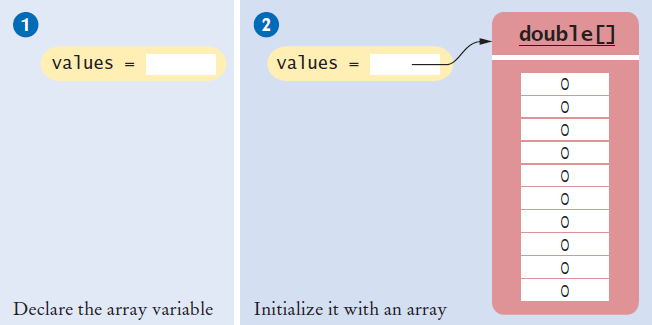
\includegraphics[height=0.25\paperheight,center]{pucrs-ep-fprog-unidade_06-arrays-laminas-declaracao_e_criacao.png}
\end{figure}
	\item O \emph{array} não pode ser utilizado até que o compilador saiba qual o tamanho do \emph{array} na etapa 2
\end{itemize}
\end{frame}

%-------------------------------------------------------
\begin{frame}\frametitle{Declarando um \emph{Array} (Etapa 1)}
\begin{itemize}
	\item As seguintes partes devem ser especificadas
\begin{figure}[h]
	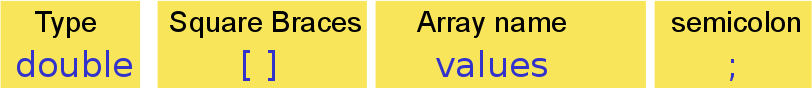
\includegraphics[height=0.10\paperheight,center]{pucrs-ep-fprog-unidade_06-arrays-laminas-declaracao_etapa_1.png}
\end{figure}
	\item Esta declaração especfica que
	\begin{itemize}
		\item Há um \emph{array} chamado \texttt{values}
		\item Que os seus elementos são do tipo \texttt{double}
		\item E que (AINDA) não foi definido quantos elementos ele poderá armazenar
	\end{itemize}
	\item Outras considerações
	\begin{itemize}
		\item \emph{Arrays} podem ser declarados  em qualquer lugar onde também seja possível declarar uma variável
		\item Não use palavras-reservadas ou nomes que já estejam em uso
	\end{itemize}
\end{itemize}
\end{frame}

%-------------------------------------------------------
\begin{frame}\frametitle{Declarando um \emph{Array} (Etapa 2)}
\begin{itemize}
	\item Reserva-se memória para todos os elementos
\begin{figure}[h]
	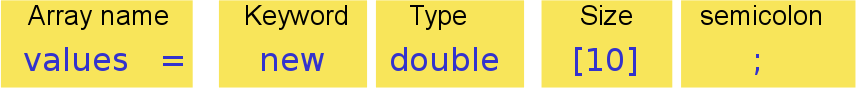
\includegraphics[height=0.10\paperheight,center]{pucrs-ep-fprog-unidade_06-arrays-laminas-declaracao_etapa_2a.png}
\end{figure}
	\item Agora o compilador sabe que o \emph{array} chamado \texttt{values} necessita de \texttt{[10]} elementos do tamanho do tipo \texttt{double}
	\item O \emph{array} também está sendo inicializado: cada elemento do \emph{array} recebe o valor 0
	\item Não se pode alterar o tamanho do \emph{array} depois da sua declaração!
\begin{figure}[h]
	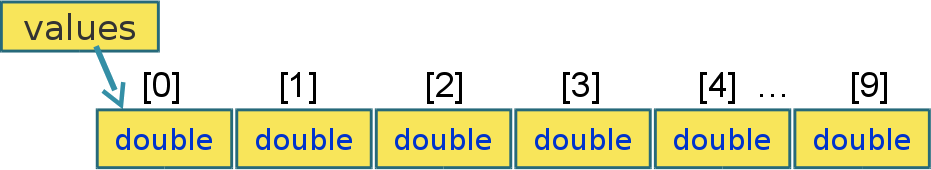
\includegraphics[height=0.15\paperheight,center]{pucrs-ep-fprog-unidade_06-arrays-laminas-declaracao_etapa_2b.png}
\end{figure}
\end{itemize}
\end{frame}

%-------------------------------------------------------
\begin{frame}\frametitle{Declaração de um \emph{Array} em uma Linha}
\begin{itemize}
	\item Declaração e criação em 1 linha
\begin{figure}[h]
	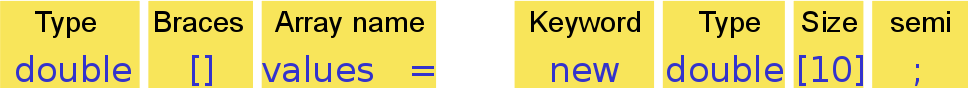
\includegraphics[height=0.10\paperheight,center]{pucrs-ep-fprog-unidade_06-arrays-laminas-declaracao_1_linha.png}
\end{figure}
	\begin{itemize}
		\item Está sendo feita a declaração de um \emph{array} chamado \texttt{values} para armazenar elementos do tipo \texttt{double}
		\item Está sendo reservada memória para armazenamento de \texttt{[10]} elementos do  tipo \texttt{double}
		\item Os elementos estão sendo inicializados com 0
	\end{itemize}
\end{itemize}
\end{frame}

%-------------------------------------------------------
\begin{frame}\frametitle{Declaração e Inicialização de um \emph{Array}}
\begin{itemize}
	\item Pode-se declarar e definir os conteúdos iniciais de todos os elementos de um \emph{array} usando:
\begin{figure}[h]
	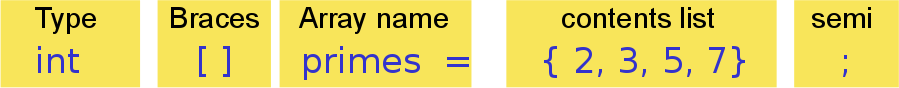
\includegraphics[height=0.10\paperheight,center]{pucrs-ep-fprog-unidade_06-arrays-laminas-declaracao_e_inicializacao.png}
\end{figure}
	\item Está sendo declarado que:
	\begin{itemize}
		\item O \emph{array} \texttt{primes} conterá elementos do tipo \texttt{int}
		\item Haverá espaço para 4 elementos (automaticamente contados pelo compilador) que conterão os seguintes valores iniciais: 2, 3, 5 e 7
		\item O par de chaves determina uma lista de valores iniciais para o \emph{array}
	\end{itemize}
\end{itemize}
\end{frame}

%-------------------------------------------------------
\begin{frame}[fragile]\frametitle{Acessando Elementos de um \emph{Array}}
\begin{itemize}
	\item Cada elemento de um \emph{array} é numerado:
	\begin{itemize}
		\item Este número é chamado de índice
		\item Acessa-se um elemento especificando o nome do \emph{array} e o índice numérico
	\end{itemize}
	\item Elementos no \emph{array} \texttt{values} são acessados por um índice inteiro \texttt{i}, usando a notação \texttt{values[i]}
\begin{columns}[T]
	\begin{column}{0.5\linewidth}
{\scriptsize
\begin{javacode}
public static void main(String[] args) {
  double[] values;
  values = new double[10];
  values[4] = 35;
}
\end{javacode}
}
	\end{column}
	\begin{column}{0.5\linewidth}
\begin{figure}[h]
	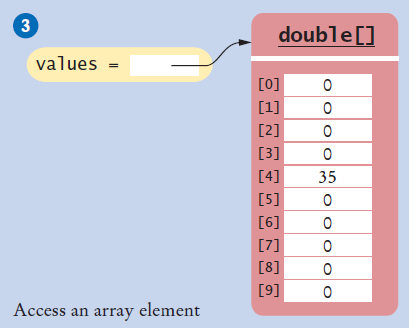
\includegraphics[height=0.35\paperheight,center]{pucrs-ep-fprog-unidade_06-arrays-laminas-acessando_elemento.png}
\end{figure}
	\end{column}
\end{columns}
\end{itemize}
\end{frame}

%-------------------------------------------------------
\begin{frame}\frametitle{Sintaxe de \emph{Arrays}}
\begin{itemize}
	\item Para declarar um \emph{array}, especifique
	\begin{itemize}
		\item O nome da variável \emph{array}
		\item O tipo de seus elementos
		\item O tamanho (número de elementos)
	\end{itemize}
\begin{figure}[h]
	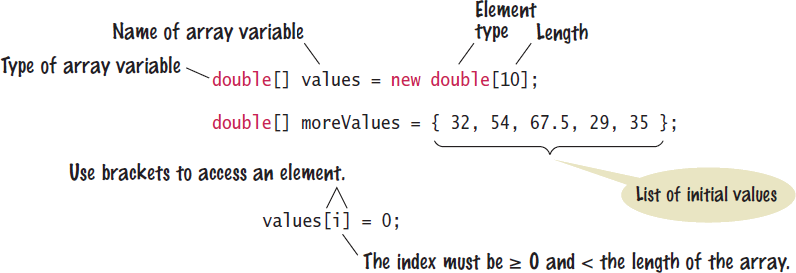
\includegraphics[height=0.45\paperheight,center]{pucrs-ep-fprog-unidade_06-arrays-laminas-sintaxe.png}
\end{figure}
\end{itemize}
\end{frame}

%-------------------------------------------------------
\begin{frame}\frametitle{Números de Índices de \emph{Arrays}}
\begin{itemize}
	\item Números de índices de \emph{arrays} iniciam em 0 e os demais são números inteiros positivos
	\item Um \emph{array} com 10 elementos tem índices de 0 até 9: \textbf{NÃO há elemento 10}
\begin{figure}[h]
	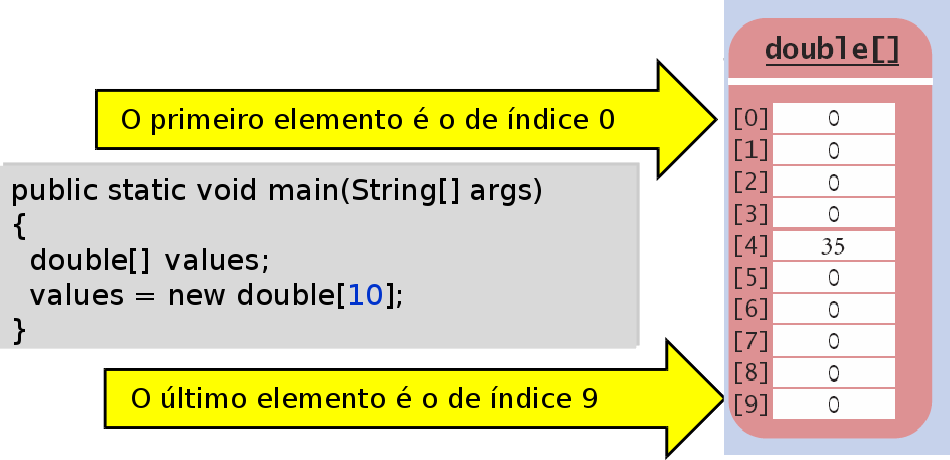
\includegraphics[height=0.5\paperheight,center]{pucrs-ep-fprog-unidade_06-arrays-laminas-indices_de_arrays.png}
\end{figure}
\end{itemize}
\end{frame}

%-------------------------------------------------------
\begin{frame}[fragile]\frametitle{Verificação de Limites de \emph{Arrays}}
\begin{itemize}
	\item Um \emph{array} sabe quantos elementos ele pode armazenar
	\begin{itemize}
		\item \texttt{values.length} é o tamanho de um \emph{array} chamado \texttt{values}
		\item Trata-se de um valor inteiro que corresponde ao índice do último elemento + 1
	\end{itemize}
	\item Usa-se isto para verificar e prevenir erros de acesso fora dos limites
	\item \emph{Strings} e \emph{arrays} usam sintaxes diferentes para encontrar os seus tamanhos
	\begin{itemize}
		\item \emph{Strings}: \texttt{name.length()}
		\item \emph{Arrays}: \texttt{values.length}
	\end{itemize}
{\scriptsize
\begin{javacode}
public static void main(String[] args) {
  int i = 10, value = 34;
  double[] values;
  values = new double[10];
  if (0 <= i && i < values.length) {  // length is 10
    values[i] = value; 
  }
}
\end{javacode}
}
\end{itemize}
\end{frame}

%-------------------------------------------------------
\begin{frame}[fragile]\frametitle{Exemplos de Declaração \emph{Arrays} (1/2)}
{\scriptsize
\begin{center}
  \begin{tabular}{|p{8cm}|p{5cm}|}
\hline
    \textbf{Declaração} & \textbf{Explicação} \\
\hline
{\scriptsize
\begin{minted}{java}
int[] numeros = new int[10];
\end{minted}
}
& Um \emph{array} de 10 inteiros. Todos os elementos inicializados com zero.\\
\hline
{\scriptsize
\begin{minted}{java}
final int TAMANHO = 10;
int[] numeros = new int[TAMANHO];
\end{minted}
}
& É uma boa ideia usar uma constante, em vez de um número constante.\\
\hline
{\scriptsize
\begin{minted}{java}
int tamanho = in.nextInt();
double[] dados = new double[tamanho];
\end{minted}
}
& O tamanho não precisa ser uma constante.\\
\hline
  \end{tabular}
\end{center}
}
\end{frame}

%-------------------------------------------------------
\begin{frame}[fragile]\frametitle{Exemplos de Declaração \emph{Arrays} (2/2)}
{\scriptsize
\begin{center}
  \begin{tabular}{|p{8cm}|p{5cm}|}
\hline
    \textbf{Declaração} & \textbf{Explicação} \\
\hline
{\scriptsize
\begin{minted}{java}
int[] quadrados = { 0, 1, 4, 9, 16 };
\end{minted}
}
& Um \emph{array} de 5 inteiros, com valores iniciais.\\
\hline
{\scriptsize
\begin{minted}{java}
String[] amigos = { "Joao", "Maria", "Paulo" };
\end{minted}
}
& Um \emph{array} com 3 \emph{strings}.\\
\hline
{\scriptsize
\begin{minted}{java}
double[] data = new int[10]; // ERRO
\end{minted}
}
& \textbf{ERRO!} Não se pode inicializar uma variável \texttt{double[]} com um \emph{array} do tipo \texttt{int[]}.\\
\hline
  \end{tabular}
\end{center}
}
\end{frame}

%-------------------------------------------------------
\begin{frame}[fragile]\frametitle{Referências a \emph{Arrays}}
\begin{itemize}
	\item É preciso perceber que há uma diferença entre:
	\begin{itemize}
		\item Variável \emph{array}: chamada de ``manipulador'' do \emph{array}
		\item Conteúdos do \emph{array}: memória onde os valores estão armazenados
	\end{itemize}
	\item Uma variável \emph{array} contém uma referência aos conteúdos do \emph{array}
	\item A referência é a localização dos conteúdos do \emph{array} (na memória)
{\footnotesize
\begin{javacode}
int[] scores = { 10, 9, 7, 4, 5 };
\end{javacode}
}
\begin{figure}[h]
	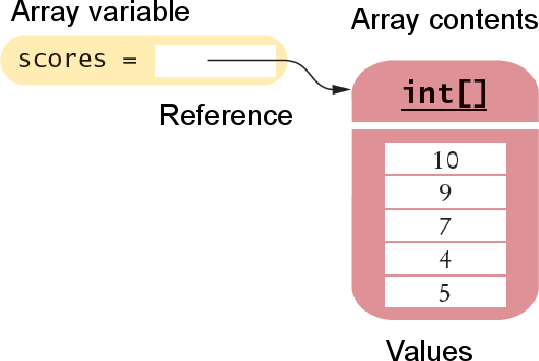
\includegraphics[height=0.3\paperheight,center]{pucrs-ep-fprog-unidade_06-arrays-laminas-referencia_a_arrays.png}
\end{figure}
\end{itemize}
\end{frame}

%-------------------------------------------------------
\begin{frame}[fragile]\frametitle{``Apelidos'' para \emph{Arrays}}
\begin{itemize}
	\item Pode-se fazer uma variável \emph{array} referenciar os mesmos conteúdos de outra variável \emph{array}
	\item Uma variável \emph{array} especifica a localização de um \emph{array}
	\item Copiar uma referência corresponde a se ter uma segunda referência para o mesmo conteúdo
{\footnotesize
\begin{javacode}
int[] resultados = { 5, 2, 8, 9, 10, 3 };
int[] valores = resultados;  // Copia da referencia do array
\end{javacode}
}
\begin{figure}[h]
	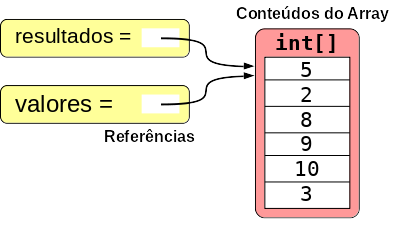
\includegraphics[height=0.3\paperheight,center]{pucrs-ep-fprog-unidade_06-arrays-laminas-apelidos_para_arrays.png}
\end{figure}
\end{itemize}
\end{frame}

%-------------------------------------------------------
\begin{frame}[fragile]\frametitle{\emph{Arrays} Parcialmente Preenchidos}
\begin{itemize}
	\item Um \emph{array} não pode ter o seu tamanho alterado durante a execução
	\begin{itemize}
		\item O programador pode necessitar obter valores até o número máximo de elementos necessário
		\item É uma boa ideia usar uma constante para o número máximo escolhido
		\item Usa-se uma variável (\texttt{tamanhoAtual} no exemplo a seguir) para controlar quantos elementos já foram obtidos
	\end{itemize}
{\footnotesize
\begin{javacode}
final int TAMANHO = 100;
double[] valores = new double[TAMANHO];
int tamanhoAtual = 0;
Scanner in = new Scanner(System.in);
while (in.hasNextDouble() && tamanhoAtual < valores.length) {
    valores[tamanhoAtual] = in.nextDouble();
    tamanhoAtual++;
}
\end{javacode}
}
\end{itemize}
\end{frame}

%-------------------------------------------------------
\begin{frame}[fragile]\frametitle{Percorrendo um \emph{Array} Parcialmente Preenchido}
\begin{itemize}
	\item No exemplo, usa-se \texttt{tamanhoAtual} (e não \texttt{valores.length}) para determinar qual o último elemento
	\item Um laço \texttt{for} é uma escolha natural para percorrer um \emph{array}
{\footnotesize
\begin{javacode}
for (int i = 0; i < tamanhoAtual; i++) {
  System.out.println(valores[i]);
}
\end{javacode}
}
\begin{figure}[h]
	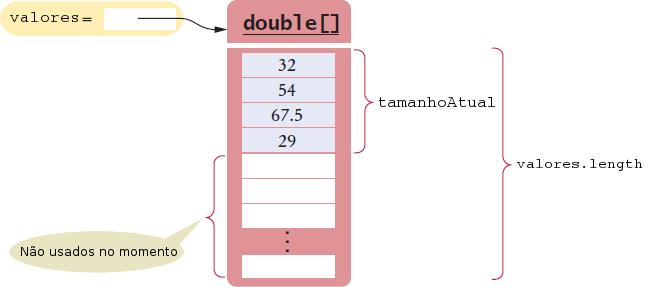
\includegraphics[height=0.3\paperheight,center]{pucrs-ep-fprog-unidade_06-arrays-laminas-percorrendo_arrays.png}
\end{figure}
\end{itemize}
\end{frame}

%-------------------------------------------------------
\begin{frame}[fragile]\frametitle{Erros Comuns (1)}
\textbf{Erro nos limites de \emph{arrays}}
\begin{itemize}
	\item Índices de \emph{arrays} iniciam em 0 e terminam em tamanho - 1
	\item Acessar um elemento que não existe é um erro bastante comum
	\item Resultado: exceção lançada em tempo de execução (\texttt{java.lang.ArrayIndexOutOfBoundsException})
{\footnotesize
\begin{javacode}
public class OutOfBounds {
  public static void main(String[] args) {
    double[] values;
    values = new double[10];
    values[10] = 100; // ERRO=EXCECAO
  }
}
\end{javacode}
}
\end{itemize}
\end{frame}

%-------------------------------------------------------
\begin{frame}[fragile]\frametitle{Erros Comuns (2)}
\textbf{\emph{Arrays} não inicializados}
\begin{itemize}
	\item Não se esqueça de inicializar variáveis \emph{array}
	\item O compilador vai gerar um erro como ``variable values might not have been initialized''
{\footnotesize
\begin{javacode}
double[] values;
...
values[0] = 29.95; // ERRO!
\end{javacode}
\begin{javacode}
double[] values;
values = new double[10];
values[0] = 29.95; // Sem erro!
\end{javacode}
}
\end{itemize}
\end{frame}

%-------------------------------------------------------
\begin{frame}[fragile]\frametitle{Exemplo: \texttt{DivisaoDeDespesas.java}}
{\tiny\inputminted[bgcolor=cyan!10]{java}{src/DivisaoDeDespesas.java}}
\end{frame}

%-------------------------------------------------------
\begin{frame}[fragile]\frametitle{Exercício}
\begin{itemize}
	\item Escreva um programa em Java para calcular a média e o desvio padrão de um conjunto de valores reais usando um vetor parcialmente preenchido com tamanho máximo igual a 100. Seu programa deve valores enquanto houver valores reais válidos na entrada ou enquanto houver espaço no vetor parcialmente preenchidos, calculando e mostrando a média e o desvio padrão desse conjunto de valores.\\
A fórmula da média é dada por:
\[ \overline{X} = \frac{\sum{x_i}}{n} \]
E a fórmula do desvio padrão é dada por:
\[ Dp = \sqrt{ \frac{ \sum{(\overline{X}-x_i)^2} }{n} } \]
\end{itemize}
\end{frame}

%-------------------------------------------------------
\begin{frame}[fragile]\frametitle{Exercício - Solução}
{\tiny\inputminted[bgcolor=cyan!10]{java}{src/DesvioPadrao.java}}
\end{frame}

%=======================================================
\section{Algoritmos Comuns para Arrays}

%-------------------------------------------------------
\begin{frame}\frametitle{Algoritmos Comuns para Arrays}
\begin{itemize}
	\item Preencher um \emph{array}
	\item Soma e média de valores
	\item Encontrar máximo e mínimo
	\item Saída de elementos com separadores
	\item Busca linear
	\item Remoção de um elemento
	\item Inserção de um elemento
	\item Troca de elementos
	\item Cópia de \emph{arrays}
	\item Aumento de tamanho de \emph{arrays}
	\item Leitura da entrada
\end{itemize}
\end{frame}

%-------------------------------------------------------
\begin{frame}[fragile]\frametitle{Preencher um \emph{Array}}
\begin{itemize}
	\item Inicializar um \emph{array} com um conjunto de valores calculados
	\item Por exemplo: preencher um \emph{array} com os quadrados de 0 até 10
\begin{javacode}
int[] quadrados = new int[11];
for (int i = 0; i < quadrados.length; i++) {
  quadrados[i] = i * i;
}
\end{javacode}
\end{itemize}
\end{frame}

%-------------------------------------------------------
\begin{frame}[fragile]\frametitle{Soma e Média de Valores}
\begin{itemize}
	\item Nunca se esqueça de evitar a divisão por zero
\begin{javacode}
if (valores.length > 0) {
   double total = 0;
   for (int i=0; i<valores.length; ++i)
      total = total + valores[i];
   double media = total / valores.length;
   System.out.println("media = " + media);
}
\end{javacode}
\end{itemize}
\end{frame}

%-------------------------------------------------------
\begin{frame}[fragile]\frametitle{Encontrar máximo e mínimo}
\begin{itemize}
	\item Defina que o maior ou menor é o primeiro elemento e teste os outros elementos usando \texttt{for}
\begin{columns}[T]
	\begin{column}{0.5\linewidth}
{\scriptsize
\begin{javacode}
// Laco tipico para encontrar o maximo
double maior = valores[0];
for (int i = 1; i < valores.length; i++)
    if  (valores[i] > maior)
        maior = valores[i];
\end{javacode}
}
	\end{column}
	\begin{column}{0.5\linewidth}
{\scriptsize
\begin{javacode}
// Laco tipico para encontrar o minimo
double menor = valores[0];
for (int i = 1; i < valores.length; i++)
    if  (valores[i] < menor)
        menor = valores[i];
\end{javacode}
}
	\end{column}
\end{columns}
	\item Às vezes também é desejável localizar o índice do maior ou menor elemento
\begin{columns}[T]
	\begin{column}{0.5\linewidth}
{\scriptsize
\begin{javacode}
// Localizar o indice do maior
int iMaior = 0;
for (int i = 1; i < valores.length; i++)
    if  (valores[i] > valores[iMaior])
        iMaior = i;
\end{javacode}
}
	\end{column}
	\begin{column}{0.5\linewidth}
{\scriptsize
\begin{javacode}
// Localizar o indice do menor
int iMenor = 0;
for (int i = 1; i < valores.length; i++)
    if  (valores[i] < valores[iMenor])
        iMenor = i;
\end{javacode}
}
	\end{column}
\end{columns}
\end{itemize}
\end{frame}

%-------------------------------------------------------
\begin{frame}[fragile]\frametitle{Saída de Elementos com Separadores}
\begin{itemize}
	\item Imprime-se o separador antes de todos os elementos, com exceção do primeiro
{\scriptsize
\begin{javacode}
double[] valores = {21, 48, 63, 30.5, 50, 18.5};
for (int i = 0; i < valores.length; i++) {
  if (i > 0) {  System.out.print(" | ");  }
  System.out.print(valores[i]);
}
System.out.println();
// Resultado: 21.0 | 48.0 | 63.0 | 30.5 | 50.0 | 18.5
\end{javacode}
}
\item Ou usa-se o método \texttt{Arrays.toString()} (muito útil para depuração)
{\scriptsize
\begin{javacode}
import java.util.Arrays;
// ...
double[] valores = {21, 48, 63, 30.5, 50, 18.5};
System.out.println(Arrays.toString(valores));
// Resultado: [21.0, 48.0, 63.0, 30.5, 50.0, 18.5]
\end{javacode}
}
\end{itemize}
\end{frame}

%-------------------------------------------------------
\begin{frame}[fragile]\frametitle{Exercício}
\begin{enumerate}
	\item Considere, por exemplo, um vetor de \texttt{String} inicializado da seguinte forma:
\begin{javacode}
String[] frutas = {"ABACATE", "BANANA", "CARAMBOLA",
                   "FIGO", "JABUTICABA"};
\end{javacode}
	escreva um laço em Java que imprima todos os itens desse array como uma lista no seguinte formato:
\begin{verbatim}
ABACATE, BANANA, CARAMBOLA, FIGO e JABUTICABA
\end{verbatim}
	use ``, '' (vírgula, espaço) depois de cada nome e `` e '' (espaço, letra e, espaço) antes do último elemento (quando ele não for o único elemento).
\end{enumerate}
\end{frame}

%-------------------------------------------------------
\begin{frame}[fragile]\frametitle{Exercício - Solução}
{\tiny\inputminted[bgcolor=cyan!10]{java}{src/Lista.java}}
\end{frame}

%-------------------------------------------------------
\begin{frame}[fragile]\frametitle{Busca Linear}
\begin{itemize}
	\item Busca-se um valor específico em um \emph{array}
	\item Inicia-se pelo primeiro elemento e para-se quando/se o valor for encontrado
	\item Usa-se uma variável booleanda \texttt{achou} para controlar o final do laço
{\scriptsize
\begin{javacode}
int valorBuscado = 100;  int pos = 0;
boolean achou = false;
while (pos < valores.length && !achou) {
   if (valores[pos] == valorBuscado) {
      achou = true;
   }
   else {
      pos++;
   }
}
if (achou)
   System.out.println("Encontrado na posicao: " + pos);
else
   System.out.println("Nao encontrado");
\end{javacode}
}
\end{itemize}
\end{frame}

%-------------------------------------------------------
\begin{frame}[fragile]\frametitle{Remoção de um Elemento}
\begin{itemize}
	\item Exige que se mantenha uma variável com o tamanho atual (número de elementos válidos)
	\item Não se pode deixar um ``buraco'' no \emph{array}
	\item Se NÃO é preciso manter o \emph{array} ordenado: copie o último elemento sobre o elemento atual e atualize o tamanho atual
\begin{columns}[T]
	\begin{column}{0.35\linewidth}
\begin{figure}[h]
	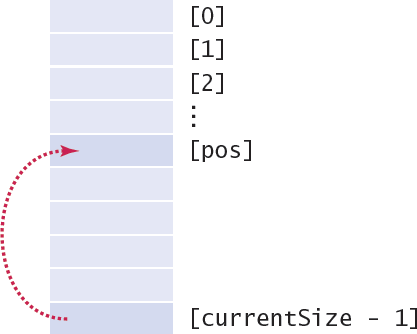
\includegraphics[height=0.35\paperheight,center]{pucrs-ep-fprog-unidade_06-arrays-laminas-remocao_a.png}
\end{figure}
	\end{column}
	\begin{column}{0.65\linewidth}
{\scriptsize
\begin{javacode}
if ( pos>=0 && pos<=valores.length-1 ) {
   if ( tamanhoAtual > 1 ) {
      valores[pos] = valores[tamanhoAtual - 1];
   }
   tamanhoAtual--;
}
\end{javacode}
}
	\end{column}
\end{columns}
\end{itemize}
\end{frame}

%-------------------------------------------------------
\begin{frame}[fragile]\frametitle{Remoção de um Elemento (Continuação)}
\begin{itemize}
	\item Se é preciso manter o \emph{array} \textbf{ordenado}: mova todos os elementos que estão após \texttt{pos} uma posição (em direção ao início do \emph{array}) e atualize o tamanho atual
\begin{columns}[T]
	\begin{column}{0.35\linewidth}
\begin{figure}[h]
	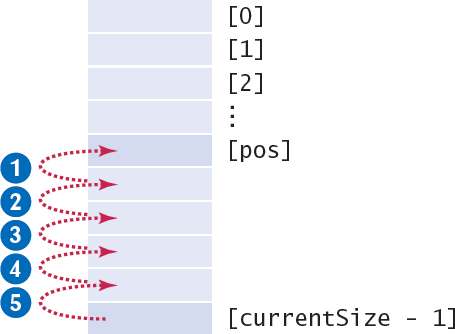
\includegraphics[height=0.35\paperheight,center]{pucrs-ep-fprog-unidade_06-arrays-laminas-remocao_b.png}
\end{figure}
	\end{column}
	\begin{column}{0.65\linewidth}
{\scriptsize
\begin{javacode}
if ( pos>=0 && pos<=valores.length-1 ) {
   for (int i = pos; i < tamanhoAtual - 1; i++) {
      valores[i] = valores[i + 1];
   }
   tamanhoAtual--;
}
\end{javacode}
}
	\end{column}
\end{columns}
\end{itemize}
\end{frame}

%-------------------------------------------------------
\begin{frame}[fragile]\frametitle{Inserção de um Elemento}
\begin{itemize}
	\item Se não é preciso manter a ordenação, apenas adiciona-se o novo valor no final e atualiza-se o tamanho
{\tiny
\begin{javacode}
if ( tamanhoAtual < valores.length ) {
   valores[tamanhoAtual] = novoValor;
   tamanhoAtual++;
}
\end{javacode}
}
	\item Se é preciso manter a ordem, localiza-se a posição correta para o novo elemento, move-se todos os elementos válidos uma posição (em direção ao final do \emph{array}) e atualiza-se o tamanho
\begin{columns}[T]
	\begin{column}{0.35\linewidth}
\begin{figure}[h]
	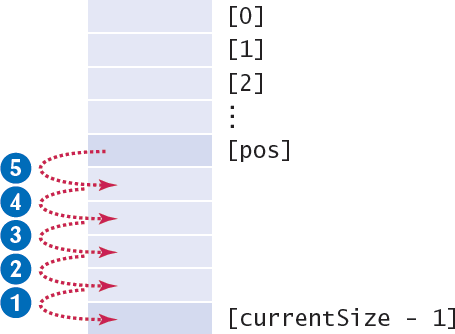
\includegraphics[height=0.30\paperheight,center]{pucrs-ep-fprog-unidade_06-arrays-laminas-insercao.png}
\end{figure}
	\end{column}
	\begin{column}{0.65\linewidth}
{\scriptsize
\begin{javacode}
if (tamanhoAtual < valores.length) {
   tamanhoAtual++;
   for (int i = tamanhoAtual - 1; i > pos; i--) {
     valores[i] = valores[i - 1];  // move p/ inicio
   }
   valores[pos] = novoValor;     // preenche buraco
}
\end{javacode}
}
	\end{column}
\end{columns}
\end{itemize}
\end{frame}

%-------------------------------------------------------
\begin{frame}[fragile]\frametitle{Troca de Elementos}
\begin{itemize}
	\item São usados 3 passos com uma variável auxiliar
\begin{columns}[T]
	\begin{column}{0.5\linewidth}
\begin{figure}[h]
	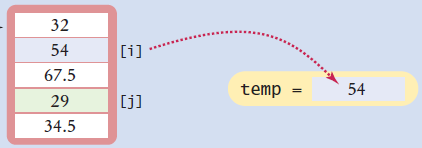
\includegraphics[height=0.20\paperheight,center]{pucrs-ep-fprog-unidade_06-arrays-laminas-swap_1.png}\\
	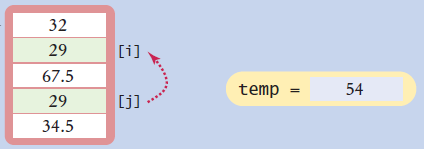
\includegraphics[height=0.20\paperheight,center]{pucrs-ep-fprog-unidade_06-arrays-laminas-swap_2.png}\\
	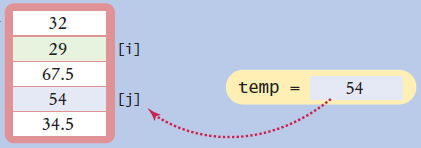
\includegraphics[height=0.20\paperheight,center]{pucrs-ep-fprog-unidade_06-arrays-laminas-swap_3.png}
\end{figure}
	\end{column}
	\begin{column}{0.5\linewidth}
\begin{javacode}
double temp = valores[i];
valores[i] = valores[j];
valores[j] = temp;  
\end{javacode}
	\end{column}
\end{columns}
\end{itemize}
\end{frame}

%-------------------------------------------------------
\begin{frame}[fragile]\frametitle{Cópia de \emph{Arrays}}
\begin{itemize}
	\item Copiar \emph{arrays} não é a mesma coisa que copiar apenas a referência
	\begin{itemize}
		\item A cópia de \emph{arrays} cria 2 conjuntos de conteúdos
		\item Exemplo de cópia de referência:
\begin{javacode}
double[] valores = { 21, 48, 63, 30.5, 50, 18.5 };
// Copia de referencia
double[] copiaRef = valores;
\end{javacode}
\begin{figure}[h]
	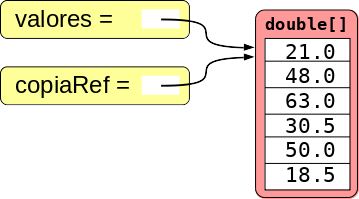
\includegraphics[height=0.30\paperheight,center]{pucrs-ep-fprog-unidade_06-arrays-laminas-copia_1.png}
\end{figure}
	\end{itemize}
\end{itemize}
\end{frame}

%-------------------------------------------------------
\begin{frame}[fragile]\frametitle{Cópia de \emph{Arrays} (2)}
\begin{itemize}
	\item Pode-se usar o método \texttt{Arrays.copyOf} (Java 6):
\begin{javacode}
double[] valores = { 21, 48, 63, 30.5, 50, 18.5 };
// copyOf cria uma nova copia, retornando a referencia
double[] copia = Arrays.copyOf(valores, valores.length);
\end{javacode}
\begin{figure}[h]
	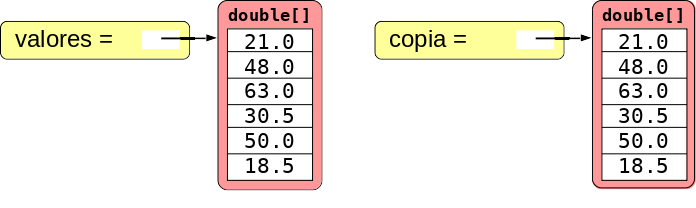
\includegraphics[height=0.30\paperheight,center]{pucrs-ep-fprog-unidade_06-arrays-laminas-copia_2.png}
\end{figure}
\end{itemize}
\end{frame}

%-------------------------------------------------------
\begin{frame}[fragile]\frametitle{Aumento de Tamanho de \emph{Arrays}}
\begin{itemize}
	\item Não é possível mudar o atributo correspondente ao tamanho de um \emph{array}, mas é possível criar outra área de memória com \texttt{copyOf} e fazer a variável \emph{array} apontar para ela
	\item Por exemplo, para duplicar o tamanho de um \emph{array} existente:
{\small
\begin{javacode}
double[] valores = { 21, 48, 63, 30.5, 50, 18.5 };
double[] aux = Arrays.copyOf(valores, 2 * valores.length);
valores = aux;
\end{javacode}
}
\end{itemize}
\end{frame}

%-------------------------------------------------------
\begin{frame}[fragile]\frametitle{Aumento de Tamanho de \emph{Arrays} (2)}
\begin{figure}[h]
	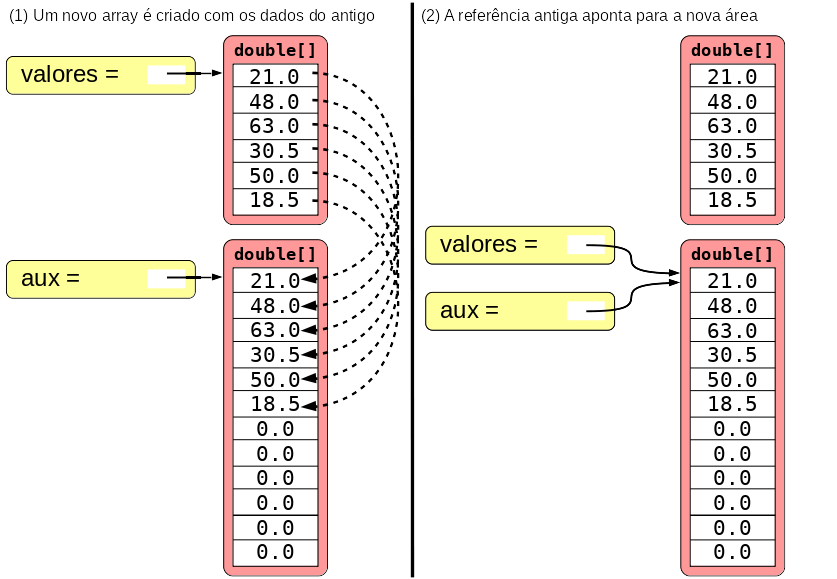
\includegraphics[height=0.75\paperheight,center]{pucrs-ep-fprog-unidade_06-arrays-laminas-aumento.png}
\end{figure}
\end{frame}

%-------------------------------------------------------
\begin{frame}[fragile]\frametitle{Leitura da Entrada}
\begin{itemize}
	\item Sabendo-se previamente o tamanho exato do \emph{array}:
{\small
\begin{javacode}
double[] entradas = new double[NUM_ENTRADAS];
for (i = 0; i < entradas.length; i++) {
   entradas[i] = in.nextDouble();
}
\end{javacode}
}
	\item Sem saber o tamanho exato, pode-se usar um tamanho máximo, mantendo-se o \emph{array} parcialmente preenchido:
{\small
\begin{javacode}
double[] entradas = new double[MAX_ENTRADAS];
int tamanhoAtual = 0;
while (in.hasNextDouble() && tamanhoAtual < entradas.length) {
   entradas[tamanhoAtual] = in.nextDouble();
   tamanhoAtual++;
}
\end{javacode}
}
\end{itemize}
\end{frame}

%-------------------------------------------------------
\begin{frame}[fragile]\frametitle{Exemplo: \texttt{MaiorDoVetor.java}}
\tiny{\inputminted[bgcolor=cyan!10]{java}{src/MaiorDoVetor.java}}
\end{frame}

%-------------------------------------------------------
\begin{frame}\frametitle{Nunca esquecer}
\begin{itemize}
	\item Subestimar o tamanho de um conjunto de dados é um erro comum
	\begin{itemize}
		\item O programador nem sempre consegue prever como as pessoas usarão o seu programa
		\item Deve-se ter o cuidado escrever código que rejeita o excesso de dados na entrada de forma elegante, principalmente quando se usa tamanhos fixos
	\end{itemize}
\end{itemize}
\end{frame}

%-------------------------------------------------------
\begin{frame}\frametitle{Exercício 1}
{\scriptsize
\begin{enumerate}
\item Construa um programa em Java que leia dados para dois vetores do tipo inteiro de 400 posições cada (\texttt{vetorA} e \texttt{vetorB}) e preencha um terceiro vetor (\texttt{vetorRes}), também de 400 posições e também do tipo inteiro, da seguinte maneira: quando o conteúdo dos elementos de mesma posição dos vetores \texttt{vetorA} e \texttt{vetorB} for igual, a posição (índice) destes elementos deve ser armazenada no vetor \texttt{vetorRes}, conforme ilustração abaixo. Devem ser utilizadas posições consecutivas de \texttt{vetorRes} para inserção dos valores desejados e, ao final do programa, devem ser escritas somente as posições preenchidas de \texttt{vetorRes}. [Adaptado do material da professora Milene Selbach Silveira]
\end{enumerate}
}
\begin{figure}[h]
	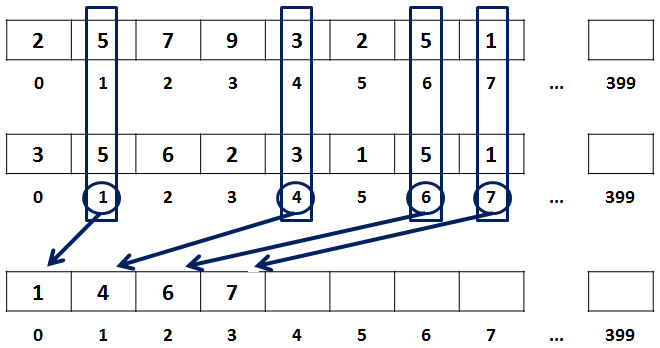
\includegraphics[height=0.40\paperheight,center]{pucrs-ep-fprog-unidade_06-arrays-laminas-exercicio.png}
\end{figure}
\end{frame}

%-------------------------------------------------------
\begin{frame}\frametitle{Exercícios 2-3}
\begin{enumerate}
\setcounter{enumi}{1}
\item Considere um \emph{array} parcialmente preenchido\\
\texttt{double[] valores = new double[100];}\\
com valores até\\
\texttt{int tamAtual;}\\
E escreva um trecho de programa em Java para eliminar todos os valores zero deste \emph{array}, sem criar um novo \emph{array}.
\item Considere um \emph{array} de inteiros chamado \texttt{valores} e escreva um programa em Java para inverter este \emph{array} (ou seja, troca o primeiro elemento pelo último, o segundo pelo penúltimo, e assim sucessivamente).
\end{enumerate}
\end{frame}

%=======================================================
\section{Usando \emph{Arrays} com Métodos}

%-------------------------------------------------------
\begin{frame}[fragile]\frametitle{Usando \emph{Arrays} com Métodos}
\begin{itemize}
	\item Métodos podem ser declarados para receber referências a \emph{arrays} como variáveis paramétricas
	\item Assim, pode-se criar um método com uma referência genérica, que receberá vetores com qualquer tamanho (do mesmo tipo, é claro)
{\tiny\inputminted[bgcolor=cyan!10]{java}{src/Somatorio.java}}
\end{itemize}
\end{frame}

%-------------------------------------------------------
\begin{frame}[fragile]\frametitle{Passando Referências}
\begin{itemize}
	\item Em Java, a passagem de parâmetros é sempre por \textbf{valor} (cópia do valor da chamada para a variável paramétrica), mas quando se passa uma referência (o que é o caso de \emph{arrays}) \textbf{é possível alterar os conteúdos desta referência} (mas NUNCA a referência propriamente dita)
{\tiny\inputminted[bgcolor=cyan!10]{java}{src/Multiplica.java}}
\end{itemize}
\end{frame}

%-------------------------------------------------------
\begin{frame}\frametitle{Passagem por Referência (1)}
\begin{itemize}
	\item As variáveis paramétricas são inicializadas com os argumentos que são passados na chamada: \texttt{v} recebe a mesma referência que \texttt{valores} e \texttt{fator} recebe 10.0
	\begin{figure}[h]
	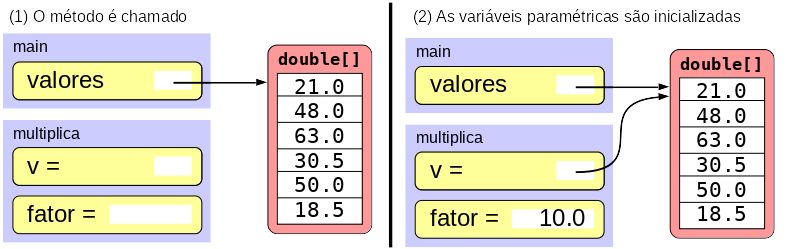
\includegraphics[height=0.4\paperheight,center]{pucrs-ep-fprog-unidade_06-arrays-laminas-passagem_por_referencia_1.png}
\end{figure}
\end{itemize}
\end{frame}

%-------------------------------------------------------
\begin{frame}\frametitle{Passagem por Referência (2)}
\begin{itemize}
	\item O método multiplica todos os elementos por 10.0
	\item O método retorna e suas variáveis paramétricas são destruídas. Entretanto, os valores do \emph{array} permanecem alterados
\begin{figure}[h]
	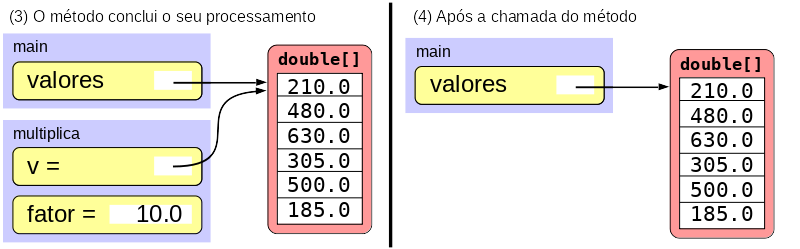
\includegraphics[height=0.4\paperheight,center]{pucrs-ep-fprog-unidade_06-arrays-laminas-passagem_por_referencia_2.png}
\end{figure}
\end{itemize}
\end{frame}

%-------------------------------------------------------
\begin{frame}[fragile]\frametitle{Método Retornando um \emph{Array}}
\begin{itemize}
	\item Métodos podem ser declarados para retornar um \emph{array} (veja, o método \texttt{quadrados()} abaixo)
	\item Ao chamar o método, deve-se atribuí-lo a uma referência que seja compatível
{\tiny\inputminted[bgcolor=cyan!10]{java}{src/Quadrados.java}}
\end{itemize}
\end{frame}

%-------------------------------------------------------
\begin{frame}[fragile]\frametitle{Exercício (1/2)}
\begin{itemize}
	\item Implemente uma classe chamada \texttt{Vetor} com uma biblioteca de métodos para processamento de vetores de inteiros
	\item Nesta classe procure implementar todos os algorimos citados até aqui
	\item Os algoritmos que ainda serão vistos poderão ser incorporados posteriormente
	\item Observe que há métodos de cada algoritmo sobrecarregados: uma versão para processamento de um vetor completo (que está pronta e chama a versão para processamento de um vetor parcialmente preenchido) e outra para processamento de um vetor parcialmente preenchido (que deverá ser implementada)
	\item Use a classe da página a seguir como modelo
	\item Defina os comentários JavaDoc para cada um dos métodos
	\item No moodle da disciplina você encontrará uma classe chamada \texttt{TestaVetor.java}, para testar a classe \texttt{Vetor.java}
\end{itemize}
\end{frame}

%-------------------------------------------------------
\begin{frame}[fragile]\frametitle{Exercício (2/2)}
\tiny{\inputminted[bgcolor=cyan!10]{java}{src/Vetor.java}}
\end{frame}

%=======================================================
\section{Tópicos Especiais}

%-------------------------------------------------------
\begin{frame}[fragile]\frametitle{Tópico Especial: Ordenação de \emph{Arrays}}
\begin{itemize}
	\item Quando se armazena valores em um \emph{array}, pode-se:
	\begin{itemize}
		\item Manter os dados desordenados (ordem aleatória)
\begin{figure}[h]
	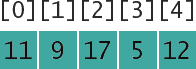
\includegraphics[height=0.10\paperheight,center]{pucrs-ep-fprog-unidade_06-arrays-laminas-ordenacao_1.png}
\end{figure}
		\item Ordená-los (de forma ascendente ou descendente)
\begin{figure}[h]
	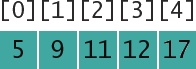
\includegraphics[height=0.10\paperheight,center]{pucrs-ep-fprog-unidade_06-arrays-laminas-ordenacao_2.png}
\end{figure}
	\end{itemize}
	\item Em um \emph{array} ordenado é muito mais fácil encontrar um valor
	\item A Java API provê um método de ordenação eficiente:
{\scriptsize
\begin{javacode}
Arrays.sort(values);      // Ordena todo o array
Arrays.sort(values, 0, currentSize);  // Parcialm. preen.
\end{javacode}
}
\end{itemize}
\end{frame}

%-------------------------------------------------------
\begin{frame}\frametitle{Tópico Especial: Algoritmos de Ordenação}
\begin{itemize}
	\item Alguns dos algoritmos de ordenação mais conhecidos são:
	\begin{itemize}
		\item \emph{Bubble Sort}: percorre os dados comparando os elementos da posição i com a posição i+1, e, se o primeiro for maior do que o segundo, inverte eles; simples; pouco eficiente
		\item \emph{Selection Sort}: procura o menor elemento e coloca na primeira posição, depois procura o segundo menor e coloca na segunda posição, e assim sucessivamente
		\item \emph{Insertion Sort}: percorre os dados da segunda posição até o final, procurando onde o elemento se encaixaria no conjunto à esquerda da posição atual (que já está ordenado); é simples e eficiente quando aplicado a pequenas listas
		\item \emph{Quick Sort}: escolhe um pivô e organiza os dados de forma que à esquerda do pivô estejam todos os valores menores do que ele, e à direita, todos os valores maiores do que o pivô, organizando a seguir as duas metades (recursivamente); é considerado o algoritmo de ordenação mais eficiente
	\end{itemize}
\end{itemize}
\end{frame}

%-------------------------------------------------------
\begin{frame}\frametitle{Tópico Especial: Pesquisa}
\begin{itemize}
	\item Já vimos um método de \textbf{pesquisa linear}
	\begin{itemize}
		\item Ele funciona sobre \emph{arrays} ordenados ou desordenados
		\item Cada elemento é visitado, partindo do início, ate que o valor procurado seja encontrado ou até que se chegue ao fim do \emph{array}
	\end{itemize}
\end{itemize}
\end{frame}

%-------------------------------------------------------
\begin{frame}\frametitle{Pesquisa Binária}
\begin{itemize}
	\item Só funciona se o \emph{array} estiver ordenado
	\item Compara o valor procurado com o elemento do meio
	\begin{itemize}
		\item Se for igual, encontrou
		\item Se for menor, desconsidera a metade superior
		\item Se for maior, desconsidera a metade inferior
	\end{itemize}
	\item Repete-se o procecimento até que o valor procurado seja encontrado ou até que não se consiga dividir o \emph{array}
\end{itemize}
\end{frame}

%-------------------------------------------------------
\begin{frame}\frametitle{Pesquisa Binária: Exemplo}
\begin{itemize}
	\item Encontrar o valor 15
\begin{figure}[h]
	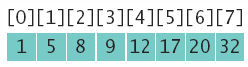
\includegraphics[height=0.10\paperheight,center]{pucrs-ep-fprog-unidade_06-arrays-laminas-pesquisa_binaria_1.png}
\end{figure}
\begin{figure}[h]
	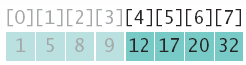
\includegraphics[height=0.10\paperheight,center]{pucrs-ep-fprog-unidade_06-arrays-laminas-pesquisa_binaria_2.png}
\end{figure}
\begin{figure}[h]
	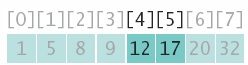
\includegraphics[height=0.10\paperheight,center]{pucrs-ep-fprog-unidade_06-arrays-laminas-pesquisa_binaria_3.png}
\end{figure}
\begin{figure}[h]
	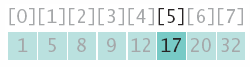
\includegraphics[height=0.10\paperheight,center]{pucrs-ep-fprog-unidade_06-arrays-laminas-pesquisa_binaria_4.png}
\end{figure}
\textbf\texttt{Sorry, 15 is not in this array.}
\end{itemize}
\end{frame}

%-------------------------------------------------------
\begin{frame}[fragile]\frametitle{Pesquisa Binária: Implementação}
{\scriptsize
\begin{javacode}
boolean found = false;
int pos = 0, low = 0, high = values.length - 1;

while (low <= high && !found) {
   pos = (low + high) / 2; // Ponto central
   if (values[pos] == searchedValue)
      found = true;        // Encontrou!
   else if (values[pos] < searchedValue) 
      low = pos + 1;       // Busca na primeira metade
   else
      high = pos - 1;      // Busca na segunda metade
}
if (found)
   System.out.println("Found at position " + pos);
else 
   System.out.println("Not found. Insert before position " + pos);
\end{javacode}
}
\end{frame}

%-------------------------------------------------------
\begin{frame}[fragile]\frametitle{Pesquisa Binária: Exercício}
{\scriptsize
Considerando o teste a seguir, monte uma tabela com colunas para cada uma das variáveis envolvidas, apresentando nas linhas os valores que estas variáveis assumem ao longo da execução. Mostre também a saída gerada. Faça 4 execuções, para \texttt{valorProc} igual a \texttt{2}, \texttt{5}, \texttt{18} e \texttt{20}.}\\
{\tiny
\begin{javacode}
boolean achou = false;
int[] valores = { 3, 5, 8, 9, 15, 16, 17, 19};
int pos = 0, inf = 0, sup = valores.length - 1;

int valorProc = in.nextInt();
while (inf <= sup && !achou) {
   pos = (inf + sup) / 2;
   if (valores[pos] == valorProc)
      achou = true;
   else if (valores[pos] < valorProc) 
      inf = pos + 1;
   else
      sup = pos - 1;
}
if (achou)
   System.out.println("pos = " + pos);
else 
   System.out.println("NAO encontrado");
\end{javacode}
}
\end{frame}

%=======================================================
\section{Solução de Problemas: Combinando Algoritmos}

%-------------------------------------------------------
\begin{frame}\frametitle{Combinando Algoritmos}
\begin{itemize}
	\item Considere o seguinte problema: o cálculo do escore de um aluno num questionário é a soma dos pontos em cada questão sem contar o menor valor.
	\item Por exemplo, para os seguintes valores:\\ \texttt{8    7    8.5    9.5    7     5    10}\\o escore final será \texttt{50}.
\end{itemize}
\end{frame}

%-------------------------------------------------------
\begin{frame}[fragile]\frametitle{Abordagem}
\begin{itemize}
	\item Decompor a tarefa em passos:
	\begin{itemize}
		\item Ler as entradas
		\item Calcular o somatório
		\item Encontrar o menor valor
		\item Subtrair o menor valor do somatório
	\end{itemize}
	\item Determinar algoritmos para cada passo e implementá-los em métodos
	\item Montar a soluçao:
{\scriptsize
\begin{javacode}
double[] scores = readInputs();
double total = sum(scores) - minimum(scores);
System.out.println("Final score: " + total);
\end{javacode}
}
	\item Revisar o código tratando soluções especiais: dados do enunciado, duas notas com o menor valor (apenas uma deve ser desconsiderada), uma única nota (escore deve ser zero), nenhuma entrada, etc.
\end{itemize}
\end{frame}

%=======================================================
\section{Solução de Problemas: Usando Objetos Reais}

%-------------------------------------------------------
\begin{frame}\frametitle{Usando Objetos Reais}
\begin{itemize}
	\item Considere o seguinte problema: você tem um \emph{array} cujo tamanho é par, e você deve trocar a primeira metade com a segunda metade
	\item Por exemplo, para um \emph{array} de 8 posições
\begin{figure}[h]
	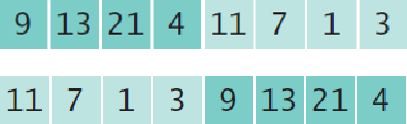
\includegraphics[height=0.15\paperheight,center]{pucrs-ep-fprog-unidade_06-arrays-laminas-troca_metades.png}
\end{figure}
	\item Uma técnica bastante útil para ajudar no desenvolvimento de algoritmos é usar objetos reais
	\item Pode-se, por exemplo, usar uma linha de objetos (moedas, cartas, pequenos brinquedos, peças de um jogo, etc.) para representar um \emph{array} e assim estudar operações necessárias na implementação de um algoritmo
\begin{figure}[h]
	
\includegraphics[height=0.1\paperheight,center]{pucrs-ep-fprog-unidade_06-arrays-laminas-moedas.png}
\end{figure}
\end{itemize}
\end{frame}

%-------------------------------------------------------
\begin{frame}\frametitle{Manipulando Objetos Reais}
\begin{itemize}
	\item Para resolver o problema proposto, os movimentos (operações) seriam::
\begin{figure}[h]
	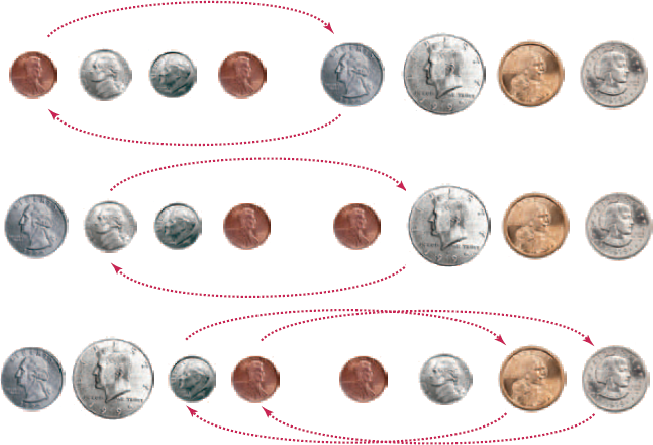
\includegraphics[height=0.50\paperheight,center]{pucrs-ep-fprog-unidade_06-arrays-laminas-algoritmo_com_moedas.png}
\end{figure}
\end{itemize}
\end{frame}

%-------------------------------------------------------
\begin{frame}\frametitle{Criando o Algoritmo}
\begin{itemize}
	\item É importante identificar:
	\begin{itemize}
		\item Quantas trocas serão necessárias?
		\item Quais os índices dos elementos que deverão ser trocados?
	\end{itemize}
	\item Estas informações devem estar relacionadas ao tamanho do \emph{array}
	\item Algoritmo:
\begin{figure}[h]
	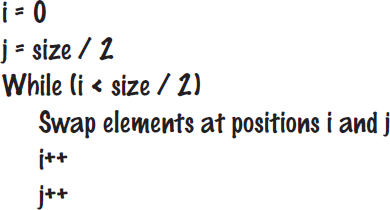
\includegraphics[height=0.3\paperheight,center]{pucrs-ep-fprog-unidade_06-arrays-laminas-algoritmo_final.png}
\end{figure}
\end{itemize}
\end{frame}

%-------------------------------------------------------
\begin{frame}\frametitle{Exercício}
Escreva um método em Java que troque a primeira metade de um \emph{array} de inteiros pela sua segunda metade. Caso o tamanho do \emph{array} seja ímpar, o método não deve fazer nada com o \emph{array}.
\end{frame}

%-------------------------------------------------------
\begin{frame}[fragile]\frametitle{Exercício (Solução)}
Escreva um método em Java que troque a primeira metade de um \emph{array} de inteiros pela sua segunda metade. Caso o tamanho do \emph{array} seja ímpar, o método não deve fazer nada com o \emph{array}.\\
{\scriptsize
\begin{javacode}
public static void trocaMetades(int[] vetor) {
   int tam = vetor.length;
   if ( tam % 2 == 0 ) {
      tam = tam / 2;
      int j = tam;
      for (int i=0; i < tam; ++i) {
         int aux = vetor[i];
         vetor[i] = vetor[j];
         vetor[j] = aux;
         j++;
      }
   }
}
\end{javacode}
}
\end{frame}

%=======================================================
\section{Arrays Bidimensionais}

%-------------------------------------------------------
\begin{frame}[fragile]\frametitle{\emph{Arrays} Bidimensionais}
\begin{itemize}
	\item \emph{Arrays} também podem ser usados para armazenar dados em duas dimensões, como dados de uma tabela
	\item Neste caso tem-se uma matriz com linhas e colunas
	\item A declaração é feita com dois pares de colchetes:
	\begin{itemize}
		\item Usando \texttt{new}:
{\scriptsize
\begin{javacode}
const int COUNTRIES = 7;
const int MEDALS = 3;
int[][] counts = new int[COUNTRIES][MEDALS];
\end{javacode}
}
		\item Usando valores inicializados e chaves (neste caso com dois ``níveis'' de chaves):
{\scriptsize
\begin{javacode}
int[][] counts = {
  { 0, 0, 1 },
  { 1, 0, 0 },
  { 0, 1, 1 },
  { 0, 1, 1 },
  { 1, 1, 0 }
};
\end{javacode}
}
	\end{itemize}
\end{itemize}
\end{frame}

%-------------------------------------------------------
\begin{frame}\frametitle{Sintaxe de \emph{Arrays} Bidimensionais}
\begin{figure}[h]
	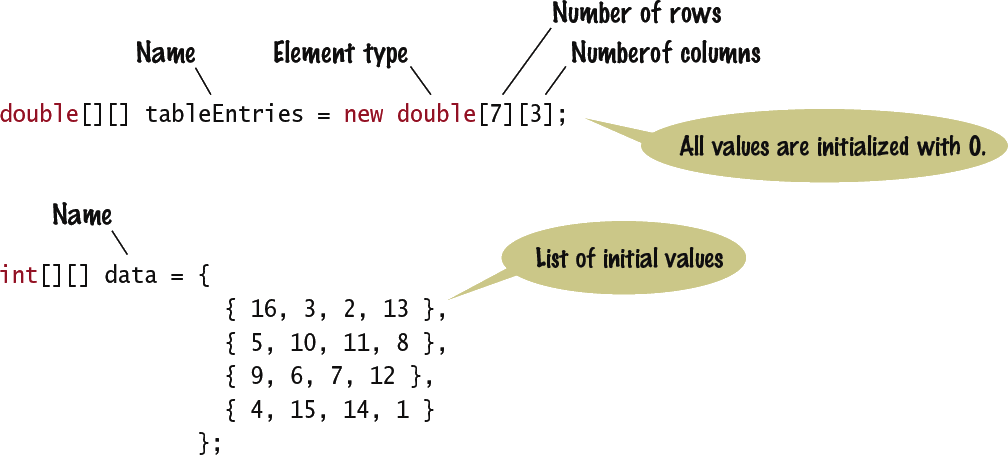
\includegraphics[height=0.5\paperheight,center]{pucrs-ep-fprog-unidade_06-arrays-laminas-array_2d_sintaxe.png}
\end{figure}
\begin{itemize}
	\item O nome do \emph{array} continua a ser a referência para os conteúdos do \emph{array}
\end{itemize}
\end{frame}

%-------------------------------------------------------
\begin{frame}[fragile]\frametitle{Acessando Elementos}
\begin{columns}[T]
	\begin{column}{0.6\linewidth}
\begin{itemize}
	\item Usa-se dois valores de índice: linha e coluna
{\scriptsize
\begin{javacode}
int value = counts[3][1];
\end{javacode}
}
	\item Para imprimir são usados 2 laços aninhados: o mais externo para linhas (i) e o mais interno para colunas (j)
{\scriptsize
\begin{javacode}
for (int i = 0; i < COUNTRIES; i++) {
   // Process the ith row
   for (int j = 0; j < MEDALS; j++) {
      // Process the jth column in the ith row
      System.out.printf("%8d", counts[i][j]);
   }
   // Start a new line at the end of the row
   System.out.println();
}
\end{javacode}
}
\end{itemize}
	\end{column}
	\begin{column}{0.4\linewidth}
\begin{figure}[h]
	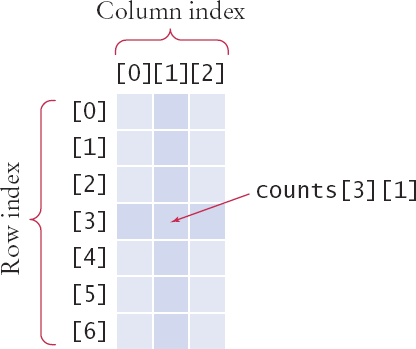
\includegraphics[height=0.5\paperheight,center]{pucrs-ep-fprog-unidade_06-arrays-laminas-array_2d_acessando_elementos.png}
\end{figure}
	\end{column}
\end{columns}
\end{frame}


%-------------------------------------------------------
\begin{frame}\frametitle{Localizando Elementos Vizinhos}
\begin{itemize}
	\item Alguns programas que trabalham com \emph{arrays} bidimensionais necessitam localizar elementos que estão em posições adjacentes, o que é muito comum em jogos
	\item Na posição \texttt{[i][j]}, os vizinhos são:
\begin{figure}[h]
	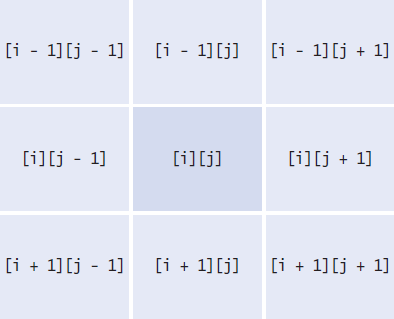
\includegraphics[height=0.4\paperheight,center]{pucrs-ep-fprog-unidade_06-arrays-laminas-array_2d_vizinhos.png}
\end{figure}
	\item Cuidado com cantos e bordas, pois não há índices negativos (posições fora do tabuleiro, por exemplo)
\end{itemize}
\end{frame}


%-------------------------------------------------------
\begin{frame}[fragile]\frametitle{Somando Linhas e Colunas}
\begin{columns}[T]
	\begin{column}{0.5\linewidth}
\begin{itemize}
	\item Soma linha \texttt{i}
\begin{figure}[h]
	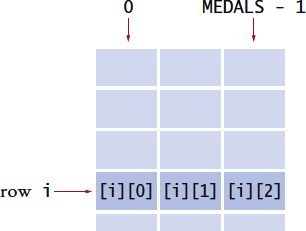
\includegraphics[height=0.3\paperheight,center]{pucrs-ep-fprog-unidade_06-arrays-laminas-array_2d_somando_linhas.png}
\end{figure}
{\scriptsize
\begin{javacode}
int total = 0;
for (int j = 0; j < MEDALS; j++) {
  total = total + counts[i][j];
}
\end{javacode}
}
\end{itemize}
	\end{column}
	\begin{column}{0.5\linewidth}
\begin{itemize}
	\item Soma coluna \texttt{j}
\begin{figure}[h]
	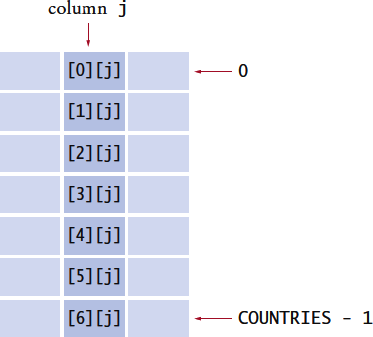
\includegraphics[height=0.4\paperheight,center]{pucrs-ep-fprog-unidade_06-arrays-laminas-array_2d_somando_colunas.png}
\end{figure}
{\scriptsize
\begin{javacode}
int total = 0;
for (int i = 0; i < COUNTRIES; i++) {
  total = total + counts[i][j];
}
\end{javacode}
}
\end{itemize}
	\end{column}
\end{columns}
\end{frame}

%-------------------------------------------------------
\begin{frame}[fragile]\frametitle{\texttt{Medals.java} {\tiny (HORSTMANN, 2013, p. 286-287)}}
{\tiny
\begin{javacode}
/**
   This program prints a table of medal winner counts with row totals.
*/
public class Medals {
   public static void main(String[] args) {
      final int COUNTRIES = 7;
      final int MEDALS = 3;
      String[] countries = {
         "Canada",
         "China",
         "Germany",
         "Korea",
         "Japan",
         "Russia",
         "United States"
      };
      int[][] counts = {
         { 1, 0, 1 },
         { 1, 1, 0 },
         { 0, 0, 1 },
         { 1, 0, 0 },
         { 0, 1, 1 },
         { 0, 1, 1 },
         { 1, 1, 0 }
      };
\end{javacode}
}
\end{frame}

%-------------------------------------------------------
\begin{frame}[fragile]\frametitle{\texttt{Medals.java} {\tiny (HORSTMANN, 2013, p. 286-287)}}
{\tiny
\begin{javacode}
      System.out.println("        Country    Gold  Silver  Bronze   Total");
      // Print countries, counts, and row totals
      for (int i = 0; i < COUNTRIES; i++) {
         // Process the ith row
         System.out.printf("%15s", countries[i]);
         int total = 0;
         // Print each row element and update the row total
         for (int j = 0; j < MEDALS; j++) {
            System.out.printf("%8d", counts[i][j]);
            total = total + counts[i][j];
         }
         // Display the row total and print a new line
         System.out.printf("%8d\n", total);
      }
   }
}
\end{javacode}
~\\
\textbf{Resultado da execução:}
\begin{verbatim}
        Country    Gold  Silver  Bronze   Total
         Canada       1       0       1       2
          China       1       1       0       2
        Germany       0       0       1       1
          Korea       1       0       0       1
          Japan       0       1       1       2
         Russia       0       1       1       2
  United States       1       1       0       2
\end{verbatim}
}
\end{frame}

%-------------------------------------------------------
\begin{frame}[fragile]	\frametitle{Dica}
\begin{itemize}
	\item Se um \emph{array} tem uma única dimensão, \texttt{length} corresponde ao tamanho desta dimensão
	\item E se \emph{array} for bidimensional? Qual o valor de \texttt{length}? Como obter o tamanho da segunda dimensão?
	\begin{itemize}
		\item Para \emph{arrays} bidimensionais, \texttt{length} retorna o número de linhas
		\item Para obter o número de colunas de uma linha, deve-se usar o \texttt{length} para a linha
{\scriptsize
\begin{javacode}
int mat[][] = new int[2][3];
System.out.println(mat.length);    // 2
System.out.println(mat[0].length); // 3
System.out.println(mat[1].length); // 3
\end{javacode}
}
	\end{itemize}
\end{itemize}
\end{frame}

%-------------------------------------------------------
\begin{frame}[fragile]\frametitle{Dica avançada}
\begin{itemize}
	\item Pode-se criar um \emph{array} com dimensões ``irregulares'' (cada linha com um número variável de elementos)
{\scriptsize
\begin{javacode}
int mat[][] = new int[2][];
mat[0] = new int[3];
mat[1] = new int[4];
System.out.println(mat.length);    // 2
System.out.println(mat[0].length); // 3
System.out.println(mat[1].length); // 4
\end{javacode}
}
\end{itemize}
\end{frame}

%-------------------------------------------------------
\begin{frame}\frametitle{Exercício 1}
Considere matrizes de inteiros com \texttt{l} linhas e \texttt{c} colunas e implemente métodos para:
\begin{enumerate}[a)]
	\item Ler todos os elementos da matriz
	\item Escrever todos os elementos da matriz
	\item Trocar a linha i1 pela linha i2 da matriz
	\item Trocar a coluna c1 pela coluna c2 da matriz
	\item Inicializar todos os elementos da matriz com valores aleatórios
\end{enumerate}
\end{frame}

%-------------------------------------------------------
\begin{frame}\frametitle{Exercício 2}
Considere matrizes quadradas de inteiros e implemente métodos para calcular:
\begin{enumerate}[a)]
	\item Somatório de todos os elementos da matriz
	\item Somatório dos elementos da linha \texttt{i} da matriz
	\item Somatório dos elementos da coluna \texttt{j} da matriz
	\item Somatório dos elementos da diagonal principal da matriz
	\item Somatório dos elementos acima da diagonal principal da matriz
	\item Somatório dos elementos abaixo da diagonal principal da matriz
	\item Somatório dos elementos da diagonal secundária da matriz
	\item Somatório dos elementos acima da diagonal secundária da matriz
	\item Somatório dos elementos abaixo da diagonal secundária da matriz
\end{enumerate}
\end{frame}

\begin{comment}
%=======================================================
\section{Arrays Lists}

%-------------------------------------------------------
\begin{frame}\frametitle{\emph{Arrays Lists}}
\begin{itemize}
	\item Quando se escreve um programa que coleta valores, nem sempre se sabe quantos elementos ele vai ter
	\item Nesta situação, um \emph{array list} de Java oferece duas vantagens significativas:
	\begin{itemize}
		\item \emph{Array lists} podem crescer e diminuir conforme a necessidade
		\item A classe \texttt{ArrayList} fornece métodos para tarefas comuns, tais como inserção e remoção de elementos
	\end{itemize}
	\item Um \emph{array list} pode se expandir para armazenar quantos elementos forem necessários
\end{itemize}
\end{frame}

%-------------------------------------------------------
\begin{frame}[fragile]\frametitle{Declarando e Usando \emph{Arrays Lists}}
\begin{itemize}
	\item A classe \texttt{ArrayList} é parte do pacote \texttt{java.util}
	\begin{itemize}
		\item É uma classe genérica (projetada para armazenar vários tipos de objetos)
	\end{itemize}
	\item O tipo dos elementos que um \emph{array list} armazena é fornecido durante a declaração:
	\begin{itemize}
		\item Dentro de \texttt{< >} como um parâmetro correspondente ao tipo
		\item O tipo deve ser uma classe
		\item Não pode ser usado para tipos primitivos (\texttt{int}, \texttt{double}, etc.)
	\end{itemize}
\begin{javacode}
ArrayList<String> names = new ArrayList<String>();
\end{javacode}
\end{itemize}
\end{frame}

%-------------------------------------------------------
\begin{frame}\frametitle{Sintaxe de \emph{Arrays Lists}}
\begin{figure}[h]
	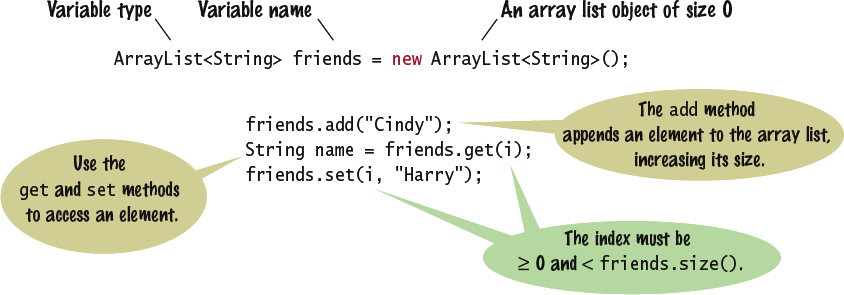
\includegraphics[height=0.35\paperheight,center]{pucrs-ep-fprog-unidade_06-arrays-laminas-arraylist_sintaxe.png}
\end{figure}
\begin{itemize}
	\item \texttt{ArrayList} provê muitos métodos úteis:
	\begin{itemize}
		\item \texttt{add}: adiciona um elemento
		\item \texttt{get}: retorna um elemento
		\item \texttt{remove}: apaga um elemento
		\item \texttt{set}: altera um elemento
		\item \texttt{size}: retorna o tamanho atual
	\end{itemize}
\end{itemize}
\end{frame}

%-------------------------------------------------------
\begin{frame}[fragile]\frametitle{Adicionando elementos com \texttt{add()}}
\begin{itemize}
	\item O método \texttt{add} tem 2 versões:
	\begin{itemize}
		\item Recebendo um novo elemento para ser adicionado no final
\begin{javacode}
names.add("Cindy");
\end{javacode}
\begin{figure}[h]
	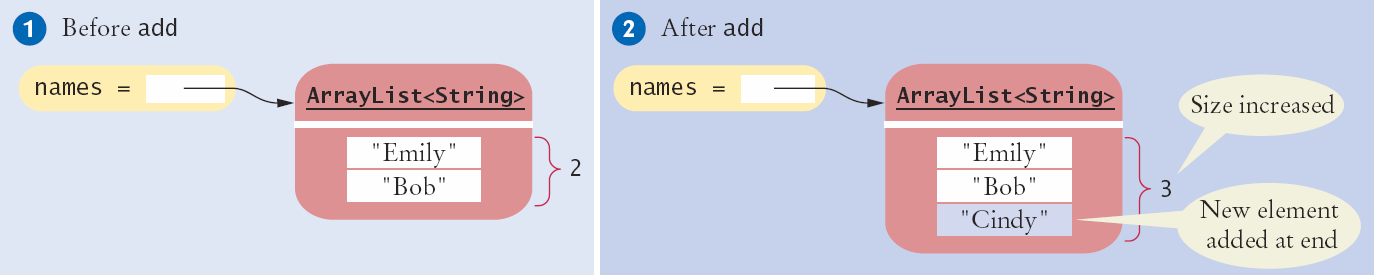
\includegraphics[height=0.3\paperheight,center]{pucrs-ep-fprog-unidade_06-arrays-laminas-arraylist_add_1.png}
\end{figure}
		\item Recebendo a localização (índice) e o novo valor a ser adicionado (o que move todos os outros elementos)
\begin{javacode}
names.add(1, "Cindy");
\end{javacode}
	\end{itemize}
\end{itemize}
\end{frame}

%-------------------------------------------------------
\begin{frame}[fragile]\frametitle{Adicionando um elemento no meio}
\begin{itemize}
	\item O método \texttt{add} recebe a localização (índice) e o novo valor a ser inserido nesta posição, e os elementos necessários são devidamente movidos
\begin{javacode}
names.add(1, "Ann");
\end{javacode}
\begin{figure}[h]
	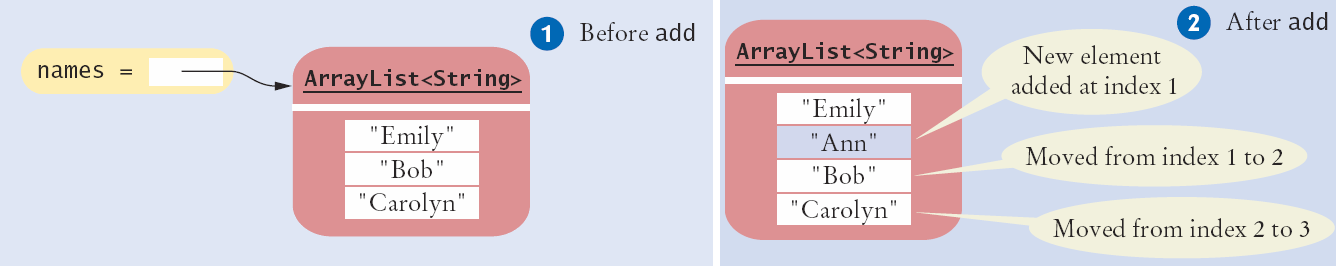
\includegraphics[height=0.3\paperheight,center]{pucrs-ep-fprog-unidade_06-arrays-laminas-arraylist_add_2.png}
\end{figure}
\end{itemize}
\end{frame}

%-------------------------------------------------------
\begin{frame}[fragile]\frametitle{Removendo um elemento}
\begin{itemize}
	\item O método \texttt{remove} recebe o localização (índice) do elemento a ser removido (os elementos necessários serão devidamente movidos)
\begin{javacode}
names.remove(1);
\end{javacode}
\begin{figure}[h]
	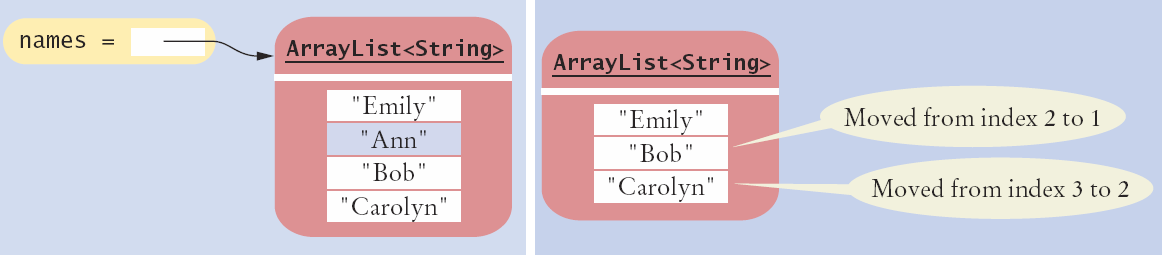
\includegraphics[height=0.3\paperheight,center]{pucrs-ep-fprog-unidade_06-arrays-laminas-arraylist_remove.png}
\end{figure}
\end{itemize}
\end{frame}

%-------------------------------------------------------
\begin{frame}[fragile]\frametitle{Usando Laços com \emph{Array Lists}}
\begin{itemize}
	\item Considerando um \emph{array list} como, por exemplo:
\begin{javacode}
ArrayList<String> letras = new ArrayList<String>();
list.add("A");    list.add("B");    list.add("C");
\end{javacode}
	\item Pode-se usar laços comuns para percorrê-lo::
\begin{javacode}
for (int i = 0; i < letras.size(); i++) {
  String letra = letras.get(i);
  System.out.println(letra);
}
\end{javacode}
	\item Ou o laço \texttt{for} abreviado:
\begin{javacode}
for (String letra : letras) {
  System.out.println(letra);
}
\end{javacode}
\end{itemize}
\end{frame}

%-------------------------------------------------------
\begin{frame}[fragile]\frametitle{Trabalhando com \emph{Array Lists}}
{\scriptsize
\begin{center}
  \begin{tabular}{|p{9cm}|p{4cm}|}
\hline
    \textbf{Código} & \textbf{Explicação} \\
\hline
\begin{javacode}
ArrayList<String> nomes = new ArrayList<String>();
\end{javacode}
& Constrói um \emph{array list} vazio que pode armazenar \emph{strings}.\\
\hline
\begin{javacode}
nomes.add("Ana");
nomes.add("Cintia");
\end{javacode}
& Adiciona elementos no final.\\
\hline
\begin{javacode}
System.out.println(nomes);
\end{javacode}
& Imprime \texttt{[Ana, Cintia]}.\\
\hline
\begin{javacode}
nomes.add(1, "Barbara");
\end{javacode}
& Insere um elemento no índice 1. \texttt{nomes} agora é \texttt{[Ana, Barbara, Cintia]}.\\
\hline
\begin{javacode}
nomes.remove(0);
\end{javacode}
& Remove o elemento de índice 0. \texttt{nomes} agora é \texttt{[Barbara, Cintia]}.\\
\hline
\begin{javacode}
nomes.set(1, "Claudia");
\end{javacode}
& Substitui um elemento por um valor diferente. \texttt{nomes} agora é \texttt{[Barbara, Claudia]}.\\
\hline
\begin{javacode}
String nome = nomes.get(i);
\end{javacode}
& Obtém um elemento.\\
\hline
\begin{javacode}
String last = nomes.get(nomes.size() - 1);
\end{javacode}
& Obtém o último elemento.\\
\hline
  \end{tabular}
\end{center}
}
\end{frame}

%-------------------------------------------------------
\begin{frame}[fragile]\frametitle{Copiando um \texttt{ArrayList}}
\begin{itemize}
	\item Uma variável \texttt{ArrayList} armazena uma referência a um \emph{array list} (da mesma forma como acontece com \emph{arrays})
	\item Para copiar uma referêcia, basta fazer:
{\scriptsize
\begin{javacode}
ArrayList<String> names = new ArrayList<String>();
names.add("Emily");    names.add("Bob");    names.add("Carolyn");
ArrayList<String> friends = names;
friends.add("Harry");
\end{javacode}
}
\begin{figure}[h]
	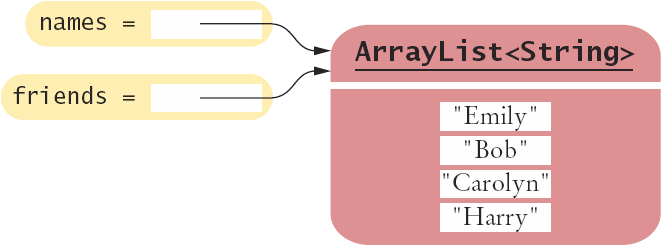
\includegraphics[height=0.18\paperheight,center]{pucrs-ep-fprog-unidade_06-arrays-laminas-arraylist_copia.png}
\end{figure}
	\item Para fazer uma cópia, passa-se a variável \texttt{ArrayList} como parâmetro para o construtor:
{\scriptsize
\begin{javacode}
ArrayList<String> newNames = new ArrayList<String>(names);
\end{javacode}
}
\end{itemize}
\end{frame}

%-------------------------------------------------------
\begin{frame}[fragile]\frametitle{\emph{Array Lists} e Métodos}
\begin{itemize}
	\item Da mesma forma que \emph{arrays}, \emph{array lists} também podem ser usadas como variáveis paramétricas e valores de retorno
	\item No exemplo a seguir, o método recebe uma lista de \emph{strings} e retorna a lista invertida
{\footnotesize
\begin{javacode}
public static ArrayList<String> reverse(ArrayList<String> names) {
  // Allocate a list to hold the method result
  ArrayList<String> result = new ArrayList<String>();
  // Traverse the names list in reverse order (last to first)
  for (int i = names.size() - 1; i >= 0; i--) {
    // Add each name to the result
    result.add(names.get(i));
  }
  return result;
}
\end{javacode}
}
\end{itemize}
\end{frame}

%-------------------------------------------------------
\begin{frame}[fragile]\frametitle{Classes Empacotadoras}
\begin{columns}[T]
	\begin{column}{0.67\linewidth}
\begin{itemize}
	\item Java provê classes empacotadoras (\emph{wrapper classes}) para os tipos primitivos de dados
	\item A conversão entre o tipo e a respectiva classe empacotadora é automática (\emph{auto-boxing})
	\begin{itemize}
		\item Tipo primitivo para classe empacotadora:
{\tiny
\begin{javacode}
double x = 29.95;
Double wrapper;
wrapper = x;  // boxing
\end{javacode}
}
\begin{figure}[h]
	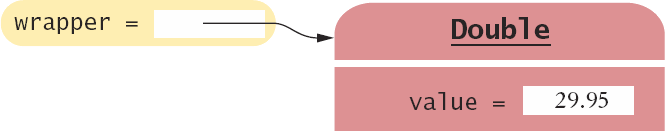
\includegraphics[height=0.12\paperheight,center]{pucrs-ep-fprog-unidade_06-arrays-laminas-wrapper_classes_1.png}
\end{figure}
		\item Classe empacotadora para tipo primitivo:
{\tiny
\begin{javacode}
double x;
Double wrapper = 29.95;
x = wrapper;  // unboxing
\end{javacode}
}
	\end{itemize}
\end{itemize}
	\end{column}
	\begin{column}{0.33\linewidth}
\begin{figure}[h]
	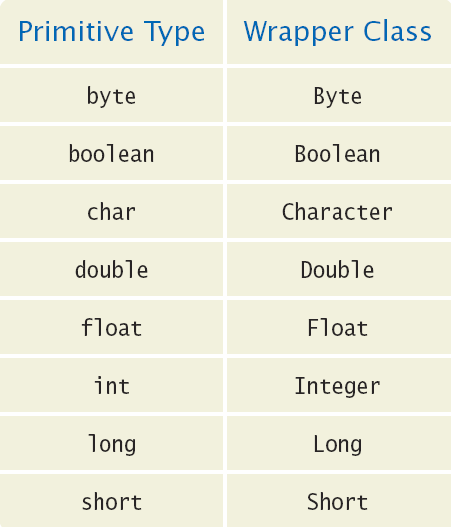
\includegraphics[height=0.6\paperheight,center]{pucrs-ep-fprog-unidade_06-arrays-laminas-wrapper_classes.png}
\end{figure}
	\end{column}
\end{columns}
\end{frame}

%-------------------------------------------------------
\begin{frame}[fragile]\frametitle{Classes Empacotadoras}
\begin{itemize}
	\item Não é possível usar tipos primitivos em um \texttt{ArrayList}, mas pode-se usar as suas classes empacotadoras
	\begin{itemize}
		\item A conversão automática (\emph{auto-boxing}) viabiliza isto
	\end{itemize}
	\item Declara-se o \texttt{ArrayList} com a respectiva classe para o tipo primitivo
	\begin{itemize}
		\item Por exemplo, com \texttt{ArrayList<Double>} pode-se adicionar variáveis ou valores \texttt{double} ao \emph{array list}
	\end{itemize}
\begin{javacode}
double x = 19.95;
ArrayList<Double> values = new ArrayList<Double>();
values.add(29.95);              // boxing
values.add(x);                  // boxing
double x = values.get(0);       // unboxing
\end{javacode}
\end{itemize}
\end{frame}

%-------------------------------------------------------
\begin{frame}[fragile]\frametitle{Algoritmos para \emph{Array Lists}}
\begin{itemize}
	\item Os algoritmos são os mesmos que se utiliza para \emph{arrays}, apenas é preciso adaptar a sintaxe
\end{itemize}
\begin{columns}[T]
	\begin{column}{0.5\linewidth}
{\scriptsize
Com \emph{arrays} usar \texttt{[i]} e \texttt{values.length}\\
\begin{javacode}
double largest = values[0];
for (int i = 1; i < values.length; i++) {
  if (values[i] > largest) {
    largest = values[i];
  }
}
\end{javacode}
}
	\end{column}
	\begin{column}{0.5\linewidth}
{\scriptsize
Com \emph{array lists} usar \texttt{get(i)} e \texttt{values.size()}\\
\begin{javacode}
double largest = values.get(0);
for (int i = 1; i < values.size(); i++) {
  if (values.get(i) > largest) {
    largest = values.get(i);
  }
}
\end{javacode}
}
	\end{column}
\end{columns}
\end{frame}

%-------------------------------------------------------
\begin{frame}\frametitle{Escolhendo entre \emph{Arrays} e \emph{Array Lists}}
\begin{itemize}
	\item Usa-se \emph{arrays} se:
	\begin{itemize}
		\item O tamanho do \emph{array} nunca se alterar
		\item Houver uma lista longa de valores primitivos e se necessita de eficiência
		\item For explicitamente solicitado
	\end{itemize}
	\item Usa-se \emph{array lists}:
	\begin{itemize}
		\item Em todos os outros casos
		\item Especialmente se o número de valores de entrada não for conhecido
	\end{itemize}
\end{itemize}
\end{frame}

%-------------------------------------------------------
\begin{frame}[fragile]\frametitle{Operações com \emph{Arrays} e \emph{Array Lists}}
\begin{center}
  \begin{tabular}{|p{5cm}|p{4cm}|p{4cm}|}
\hline
    \textbf{Operação} & \textbf\emph{Arrays} & \textbf\emph{Array Lists}\\
\hline
Obter um elemento. &
\begin{javacode}
x = values[4];
\end{javacode}
&
\begin{javacode}
x = values.get(4);
\end{javacode}
\\
\hline
Substituir um elemento. &
\begin{javacode}
values[4] = 35;
\end{javacode}
&
\begin{javacode}
values.set(4,35);
\end{javacode}
\\
\hline
Número de elementos. &
\begin{javacode}
values.length
\end{javacode}
&
\begin{javacode}
values.size()
\end{javacode}
\\
\hline
Número de elementos preenchidos. &
\begin{javacode}
currentSize
\end{javacode}
&
\begin{javacode}
values.size()
\end{javacode}
\\
\hline
Remover um elemento. &
[Algoritmo]
&
\begin{javacode}
values.remove(4);
\end{javacode}
\\
\hline
Adicionar um elemento, aumentando a coleção. &
[Algoritmo]
&
\begin{javacode}
values.add(35);
\end{javacode}
\\
\hline
Inicializar uma coleção. &
\begin{javacode}
int[] values = {
  1, 4, 9
};
\end{javacode}
&
Usar \texttt{add} várias vezes.
\\
\hline
  \end{tabular}
\end{center}
\end{frame}

%-------------------------------------------------------
\begin{frame}\frametitle{Erro Comum}
\begin{itemize}
	\item \texttt{length} \emph{versus} \texttt{size}
	\begin{itemize}
		\item Infelizmente, a sintaxe de Java para determinar o número de elementos em um \emph{array}, em um \emph{array list} e em um \emph{string} é diferente
		\item É um erro comum confundir as formas
	\end{itemize}
\begin{figure}[h]
	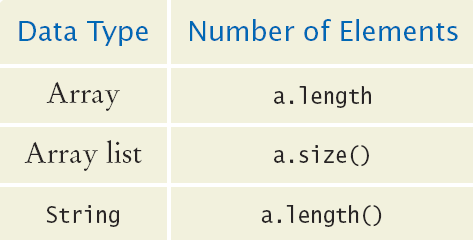
\includegraphics[height=0.3\paperheight,center]{pucrs-ep-fprog-unidade_06-arrays-laminas-length_size.png}
\end{figure}
\end{itemize}
\end{frame}
\end{comment}

%=======================================================
\section{Argumentos da Linha de Comando}

%-------------------------------------------------------
\begin{frame}[fragile]\frametitle{Argumentos da Linha de Comando}
\begin{itemize}
	\item Pode-se parametrizar a execução de programas através de argumentos da linha de comandos
	\item Por exemplo, opções, dados ou nomes de arquivos são frequentemente fornecidos após o nome do programa na linha de comandos (\emph{prompt}):
{\scriptsize
\begin{verbatim}
java Argumentos -v um dois "3 quatro 5"
\end{verbatim}
}
	\item Java provê acesso a estas informações através de um \emph{array} de \emph{strings} chamado \texttt{args} passado como parâmetro para o método \texttt{main}:
{\scriptsize
\begin{javacode}
public static void main(String[] args)
\end{javacode}
}
	\item Cada elemento de \texttt{args} corresponde a uma palavra digitada na linha de comandos após o nome do programa
	\item \texttt{args.length} contém, portanto, o número de argumentos
{\scriptsize
\begin{javacode}
args.length = 4
args[0] = "-v"
args[1] = "um"
args[2] = "dois"
args[3] = "3 quatro 5"
\end{javacode}
}
	\item Tradicionalmente opções costum iniciar com um sinal de menos (\texttt{'-'})
\end{itemize}
\end{frame}

%-------------------------------------------------------
\begin{frame}[fragile]\frametitle{\texttt{Argumentos.java}}
\tiny{\inputminted[bgcolor=cyan!10]{java}{src/Argumentos.java}}
\end{frame}

%=======================================================
\section{Sumário}

%-------------------------------------------------------
\begin{frame}\frametitle{Sumário: \emph{Arrays}}
\begin{itemize}
	\item Um \emph{array} armazena uma sequência de valores do mesmo tipo
	\item Elementos individuais em um \emph{array} são acessados por um índice inteiro \texttt{i}, usando a notação \texttt{values[i]}
	\item Um elemento de \emph{array} pode ser usado como qualquer outra variável
	\item Um índice de \emph{array} deve ser no mínimo 0 e menor do que o tamanho do \emph{array}
	\item Um erro de limite, que ocorre se você não especificar um índice válido de \emph{array}, pode abortar a execução do programa
	\item Use a expressão \texttt{array.length} para encontrar o número de elementos de um \emph{array}
	\item Uma referência de \emph{array} armazena o endereço do local do conteúdo do \emph{array}
	\item Copiar uma referência cria uma segunda referência para o mesmo \emph{array}
	\item Com \emph{arrays} parcialmente preenchidos, deve-se manter uma variável auxiliar com o tamanho atual do \emph{array}
\end{itemize}
\end{frame}

%-------------------------------------------------------
\begin{frame}\frametitle{Sumário: \emph{Arrays}}
\begin{itemize}
	\item Uma pesquisa linear inspeciona os elementos em sequência até encontrar o elemento procurado
	\item Usa-se uma variável temporária quando elementos devem ser trocados
	\item Usa-se o método \texttt{Arrays.copyOf} para copiar os elementos de um \emph{array} para um novo \emph{array}
	\item \emph{Arrays} podem ser usados como variáveis paramétricas de métodos e podem ser retornados por métodos
\end{itemize}
\end{frame}

%-------------------------------------------------------
\begin{frame}\frametitle{Sumário: \emph{Arrays}}
\begin{itemize}
	\item Pode-se resolver tarefas complexas combinando algoritmos básicos
	\item Deve-se conhecer os algoritmos básicos para reaproveitá-los e, quando necessário, adaptá-los 
	\item Pode-se usar objetos reais para auxiliar no desenvolvimento de algoritmos
	\item Usa-se \emph{arrays} bidimensionais (matrizes) para armazenar dados de tabelas
	\item Elementos individuais de um \emph{array} bidimensional são acessados usando dois valores de índice: \texttt{values[i][j]}
	\item Programas iniciados a partir da linha de comandos recebem argumentos da linha de comandos através de argumentos do método \texttt{main()}
\end{itemize}
\end{frame}

\begin{comment}
%-------------------------------------------------------
\begin{frame}\frametitle{Sumário: \emph{Array Lists}}
\begin{itemize}
	\item Um \emph{array list} armazena uma sequência de valores cujo número pode-se alterar
	\begin{itemize}
		\item A classe \texttt{ArrayList} é uma classe genérica: \texttt{ArrayList<Type>} armazena elementos do tipo especificado
		\item Usa-se o método \texttt{size} para obter o tamanho atual do \emph{array list}
		\item Use os métodos \texttt{get} e \texttt{set} para acessar elementos de um \emph{array list} de determinado índice
		\item Use os métodos \texttt{add} e \texttt{remove} para adicionar e remover elementos de um \emph{array list}
	\end{itemize}
	\item Para armazenar tipos primitivos em \emph{array lists}, deve-se usar classes empacotadoras (\emph{wrapper classes}): \texttt{Boolean}, \texttt{Byte}, \texttt{Character}, \texttt{Double}, \texttt{Float}, \texttt{Integer}, \texttt{Long}, \texttt{Short}
\end{itemize}
\end{frame}
\end{comment}

%=======================================================
\section{Humor}

%-------------------------------------------------------
\begin{frame}\frametitle{Vida de Programador {\tiny (NOEL, 2016, p. 37)}}
\begin{figure}[h]
	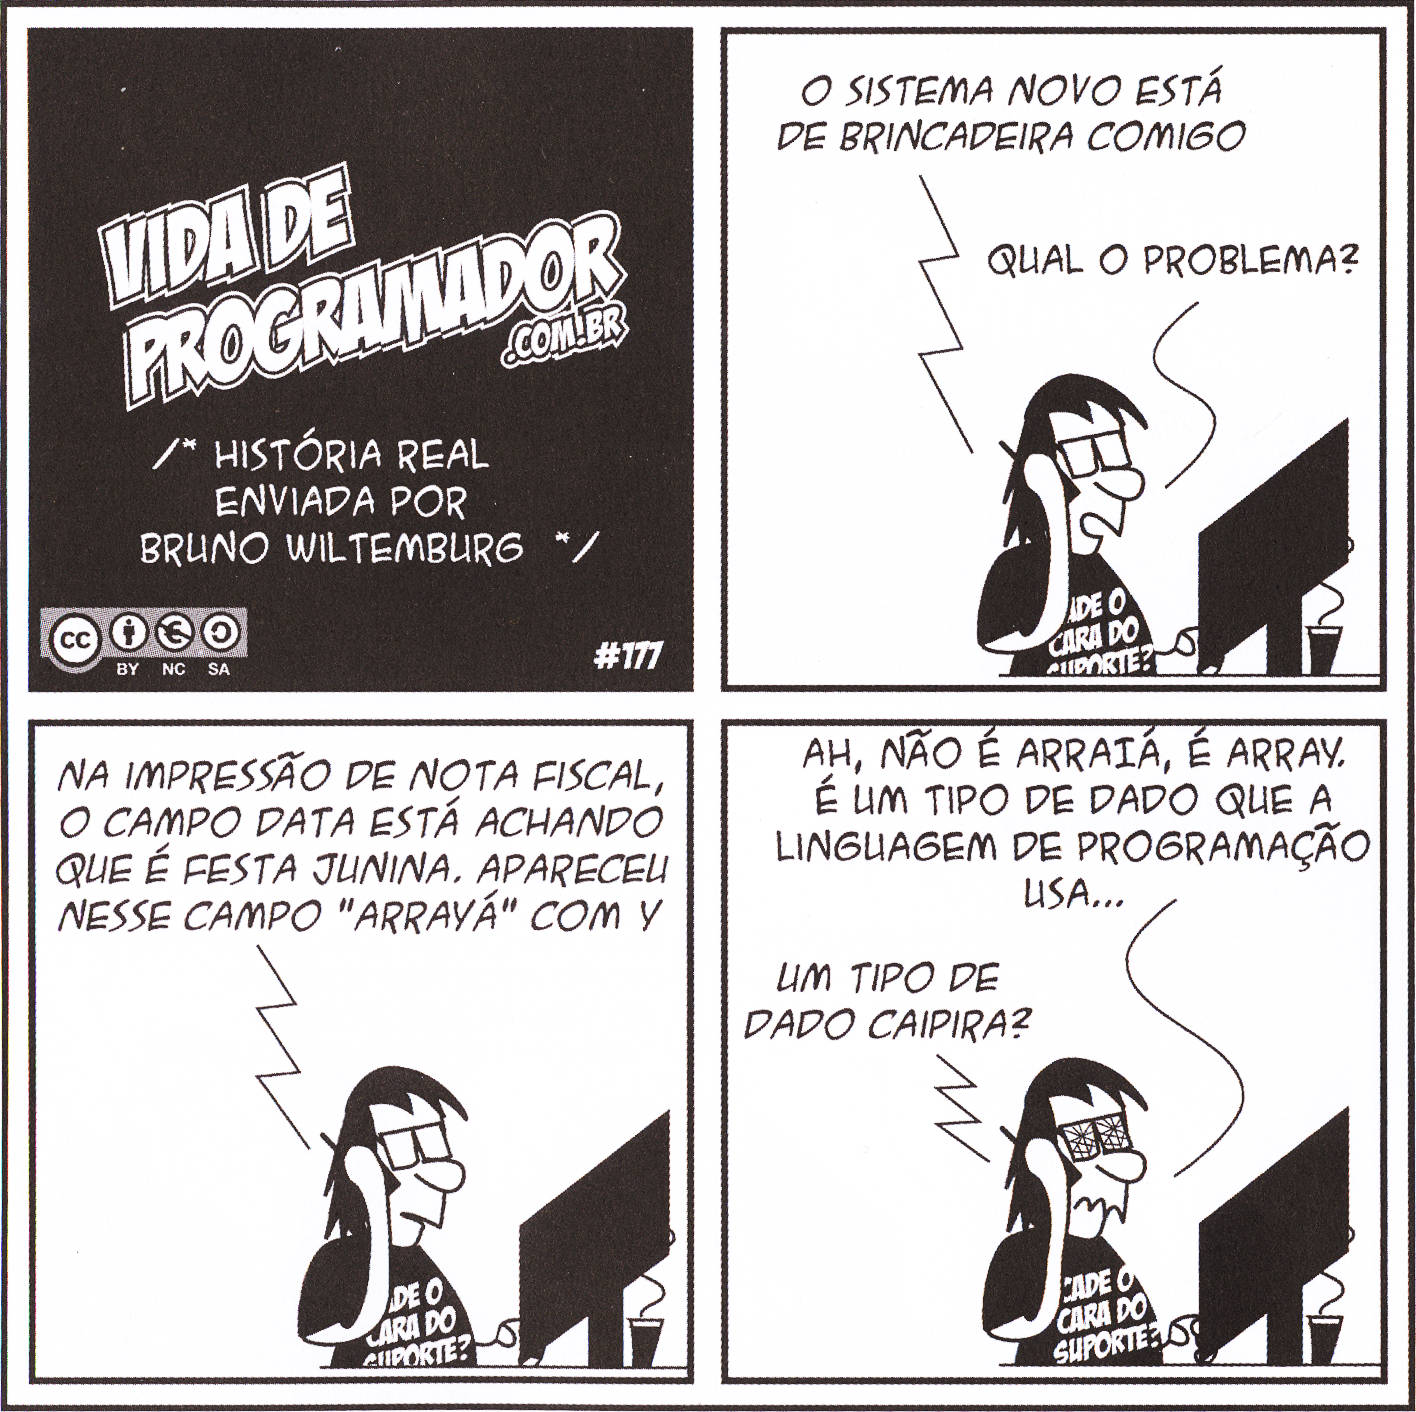
\includegraphics[height=0.7\paperheight,center]{pucrs-ep-fprog-unidade_06-arrays-laminas-vida_de_programador.jpg}
\end{figure}
\end{frame}

%=======================================================
\section{Tópicos Complementares}

%-------------------------------------------------------
\begin{frame}[fragile]\frametitle{O Laço \texttt{for} Abreviado }
\begin{itemize}
	\item Usar laços \texttt{for} para percorrer um \emph{array} é bastante comum:
	\begin{itemize}
		\item O \texttt{for} abreviado simplifica este processo
		\item Este laço também é chamado de \emph{for each} (``para cada '')
		\item Este código pode ser lido como: ``Para cada elemento do \emph{array}''
	\end{itemize}
	\item À medida que o laço avança, ele:
	\begin{itemize}
		\item Acessará cada elemento sequencialmente (de 0 até o tamanho -1)
		\item Copiará o seu valor para a variável de induçao
		\item Executará o corpo do laço
	\end{itemize}
	\item Não é possível para:
	\begin{itemize}
		\item Alterar elementos
		\item Obter erros de limite
	\end{itemize}
{\scriptsize
\begin{javacode}
double[] values = ...;
double total = 0;
for (double element : values) {
  total = total + element;
}
\end{javacode}
}
\end{itemize}
\end{frame}

%-------------------------------------------------------
\begin{frame}\frametitle{Sintaxe do \texttt{for} abreviado }
\begin{itemize}
	\item Use o \texttt{for} abreviado quando:
	\begin{itemize}
		\item For necessário acessar cada elemento de um \emph{array}
		\item Não for necessário alterar qualquer elemento do \emph{array}
	\end{itemize}
\begin{figure}[h]
	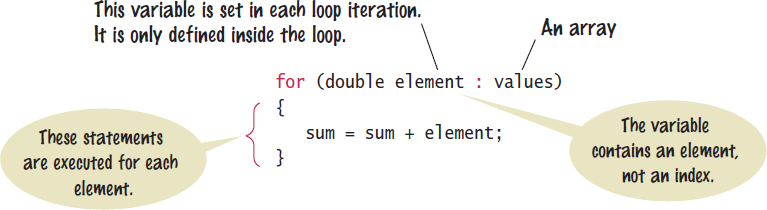
\includegraphics[height=0.4\paperheight,center]{pucrs-ep-fprog-unidade_06-arrays-laminas-sintaxe_for_abreviado.png}
\end{figure}
\end{itemize}
\end{frame}

%=======================================================
\section{Referências}

%-------------------------------------------------------
\begin{frame}\frametitle{Referências}
\noindent{HORSTMANN, C. \textbf{Java for Everyone – Late Objects}. 2. ed. Hoboken: Wiley, 2013. xxxiv, 589 p.}\\
~\\
\noindent{NOEL, Andre. \textbf{Vida de Programador.com.br - Volume 1}. São Paulo: Novatec, 2016. 118 p.}
\end{frame}

%=======================================================
\end{document}

